\documentclass[11pt,addpoints,answers]{exam}

%-----------------------------------------------------------------------------
% PACKAGES AND OTHER DOCUMENT CONFIGURATIONS
%-----------------------------------------------------------------------------

\usepackage[margin=1in]{geometry}
\usepackage{amsmath, amsfonts}
\usepackage{enumerate}
\usepackage{graphicx}
\usepackage{titling}
\usepackage{url}
\usepackage{xfrac}
\usepackage{natbib}
\usepackage{amssymb}
\usepackage{amsthm}
\usepackage{paralist}
\usepackage{epstopdf}
\usepackage{tabularx}
\usepackage{longtable}
\usepackage{multirow}
\usepackage{multicol}
\usepackage[colorlinks=true,urlcolor=blue]{hyperref}
\usepackage{algorithm}
\usepackage{algorithmicx}
\usepackage[noend]{algpseudocode}
\usepackage{float}
\usepackage{enumerate}
\usepackage{array}
\usepackage{environ}
\usepackage{times}
\usepackage{textcomp}
\usepackage{caption}
\usepackage{parskip} % For NIPS style paragraphs.
\usepackage[compact]{titlesec} % Less whitespace around titles
\usepackage[inline]{enumitem} % For inline enumerate* and itemize*
\usepackage{datetime}
\usepackage{comment}
% \usepackage{minted}
\usepackage{lastpage}
\usepackage{color}
\usepackage{xcolor}
\usepackage[final]{listings}
\usepackage{tikz}
\usetikzlibrary{shapes,decorations}
\usepackage{framed}
\usepackage{booktabs}
\usepackage{cprotect}
\usepackage{verbatim}
\usepackage{verbatimbox}
\usepackage{multicol}
\usepackage{hyperref}
\usepackage{subcaption}
\usepackage{mathtools} % For drcases
\usepackage{cancel}
\usepackage[many]{tcolorbox}
\usepackage{soul}
\usepackage[bottom]{footmisc}
\usepackage{bm}
\usepackage{wasysym}
\usepackage[utf8]{inputenc}
\usepackage{tikz}
\usetikzlibrary{arrows}
\usetikzlibrary{arrows.meta}
\usetikzlibrary{shapes.geometric}
\usetikzlibrary{positioning, arrows, automata, calc}
\usepackage{transparent}

\newtcolorbox[]{your_solution}[1][]{
    % breakable,
    enhanced,
    nobeforeafter,
    colback=white,
    title=Your Answer,
    sidebyside align=top,
    box align=top,
    #1
}

%%%%%%%%%%%%%%%%%%%%%%%%%%%%%%%%%%%%%%%%%%%
% Formatting for \CorrectChoice of "exam" %
%%%%%%%%%%%%%%%%%%%%%%%%%%%%%%%%%%%%%%%%%%%

\CorrectChoiceEmphasis{}
\checkedchar{\blackcircle}

%%%%%%%%%%%%%%%%%%%%%%%%%%%%%%%%%%%%%%%%%%%
% Rotated Column Headers                  %
%%%%%%%%%%%%%%%%%%%%%%%%%%%%%%%%%%%%%%%%%%%
\usepackage{adjustbox}
\usepackage{array}

%https://tex.stackexchange.com/questions/32683/rotated-column-titles-in-tabular

\newcolumntype{R}[2]{%
    >{\adjustbox{angle=#1,lap=\width-(#2)}\bgroup}%
    l%
    <{\egroup}%
}
\newcommand*\rot{\multicolumn{1}{R{45}{1em}}}% no optional argument here, please!

%%%%%%%%%%%%%%%%%%%%%%%%%%%%%%%%%%%%%%%%%%
% Custom commands                        %
%%%%%%%%%%%%%%%%%%%%%%%%%%%%%%%%%%%%%%%%%%

\newcommand{\vc}[1]{\boldsymbol{#1}}
\newcommand{\adj}[1]{\frac{d J}{d #1}}
\newcommand{\chain}[2]{\adj{#2} = \adj{#1}\frac{d #1}{d #2}}

\newcommand{\R}{\mathbb{R}}
\newcommand{\blackcircle}{\tikz\draw[black,fill=black] (0,0) circle (1ex);}
\renewcommand{\circle}{\tikz\draw[black] (0,0) circle (1ex);}

\newcommand{\emptysquare}{{\LARGE $\square$}\ \ }
\newcommand{\filledsquare}{{\LARGE $\blacksquare$}\ \ }
\newcommand{\emptycircle}{{\LARGE $\fullmoon$}\ \ }
\newcommand{\filledcircle}{{\LARGE $\newmoon$}\ \ }

\newcommand{\ntset}{test}

% mathcal
\newcommand{\Ac}{\mathcal{A}}
\newcommand{\Bc}{\mathcal{B}}
\newcommand{\Cc}{\mathcal{C}}
\newcommand{\Dc}{\mathcal{D}}
\newcommand{\Ec}{\mathcal{E}}
\newcommand{\Fc}{\mathcal{F}}
\newcommand{\Gc}{\mathcal{G}}
\newcommand{\Hc}{\mathcal{H}}
\newcommand{\Ic}{\mathcal{I}}
\newcommand{\Jc}{\mathcal{J}}
\newcommand{\Kc}{\mathcal{K}}
\newcommand{\Lc}{\mathcal{L}}
\newcommand{\Mc}{\mathcal{M}}
\newcommand{\Nc}{\mathcal{N}}
\newcommand{\Oc}{\mathcal{O}}
\newcommand{\Pc}{\mathcal{P}}
\newcommand{\Qc}{\mathcal{Q}}
\newcommand{\Rc}{\mathcal{R}}
\newcommand{\Sc}{\mathcal{S}}
\newcommand{\Tc}{\mathcal{T}}
\newcommand{\Uc}{\mathcal{U}}
\newcommand{\Vc}{\mathcal{V}}
\newcommand{\Wc}{\mathcal{W}}
\newcommand{\Xc}{\mathcal{X}}
\newcommand{\Yc}{\mathcal{Y}}
\newcommand{\Zc}{\mathcal{Z}}

% mathbb
\newcommand{\Ab}{\mathbb{A}}
\newcommand{\Bb}{\mathbb{B}}
\newcommand{\Cb}{\mathbb{C}}
\newcommand{\Db}{\mathbb{D}}
\newcommand{\Eb}{\mathbb{E}}
\newcommand{\Fb}{\mathbb{F}}
\newcommand{\Gb}{\mathbb{G}}
\newcommand{\Hb}{\mathbb{H}}
\newcommand{\Ib}{\mathbb{I}}
\newcommand{\Jb}{\mathbb{J}}
\newcommand{\Kb}{\mathbb{K}}
\newcommand{\Lb}{\mathbb{L}}
\newcommand{\Mb}{\mathbb{M}}
\newcommand{\Nb}{\mathbb{N}}
\newcommand{\Ob}{\mathbb{O}}
\newcommand{\Pb}{\mathbb{P}}
\newcommand{\Qb}{\mathbb{Q}}
\newcommand{\Rb}{\mathbb{R}}
\newcommand{\Sb}{\mathbb{S}}
\newcommand{\Tb}{\mathbb{T}}
\newcommand{\Ub}{\mathbb{U}}
\newcommand{\Vb}{\mathbb{V}}
\newcommand{\Wb}{\mathbb{W}}
\newcommand{\Xb}{\mathbb{X}}
\newcommand{\Yb}{\mathbb{Y}}
\newcommand{\Zb}{\mathbb{Z}}

% mathbf lowercase
\newcommand{\av}{\mathbf{a}}
\newcommand{\bv}{\mathbf{b}}
\newcommand{\cv}{\mathbf{c}}
\newcommand{\dv}{\mathbf{d}}
\newcommand{\ev}{\mathbf{e}}
\newcommand{\fv}{\mathbf{f}}
\newcommand{\gv}{\mathbf{g}}
\newcommand{\hv}{\mathbf{h}}
\newcommand{\iv}{\mathbf{i}}
\newcommand{\jv}{\mathbf{j}}
\newcommand{\kv}{\mathbf{k}}
\newcommand{\lv}{\mathbf{l}}
\newcommand{\mv}{\mathbf{m}}
\newcommand{\nv}{\mathbf{n}}
\newcommand{\ov}{\mathbf{o}}
\newcommand{\pv}{\mathbf{p}}
\newcommand{\qv}{\mathbf{q}}
\newcommand{\rv}{\mathbf{r}}
\newcommand{\sv}{\mathbf{s}}
\newcommand{\tv}{\mathbf{t}}
\newcommand{\uv}{\mathbf{u}}
\newcommand{\vv}{\mathbf{v}}
\newcommand{\wv}{\mathbf{w}}
\newcommand{\xv}{\mathbf{x}}
\newcommand{\yv}{\mathbf{y}}
\newcommand{\zv}{\mathbf{z}}

% mathbf uppercase
\newcommand{\Av}{\mathbf{A}}
\newcommand{\Bv}{\mathbf{B}}
\newcommand{\Cv}{\mathbf{C}}
\newcommand{\Dv}{\mathbf{D}}
\newcommand{\Ev}{\mathbf{E}}
\newcommand{\Fv}{\mathbf{F}}
\newcommand{\Gv}{\mathbf{G}}
\newcommand{\Hv}{\mathbf{H}}
\newcommand{\Iv}{\mathbf{I}}
\newcommand{\Jv}{\mathbf{J}}
\newcommand{\Kv}{\mathbf{K}}
\newcommand{\Lv}{\mathbf{L}}
\newcommand{\Mv}{\mathbf{M}}
\newcommand{\Nv}{\mathbf{N}}
\newcommand{\Ov}{\mathbf{O}}
\newcommand{\Pv}{\mathbf{P}}
\newcommand{\Qv}{\mathbf{Q}}
\newcommand{\Rv}{\mathbf{R}}
\newcommand{\Sv}{\mathbf{S}}
\newcommand{\Tv}{\mathbf{T}}
\newcommand{\Uv}{\mathbf{U}}
\newcommand{\Vv}{\mathbf{V}}
\newcommand{\Wv}{\mathbf{W}}
\newcommand{\Xv}{\mathbf{X}}
\newcommand{\Yv}{\mathbf{Y}}
\newcommand{\Zv}{\mathbf{Z}}

% bold greek lowercase
\newcommand{\alphav     }{\boldsymbol \alpha     }
\newcommand{\betav      }{\boldsymbol \beta      }
\newcommand{\gammav     }{\boldsymbol \gamma     }
\newcommand{\deltav     }{\boldsymbol \delta     }
\newcommand{\epsilonv   }{\boldsymbol \epsilon   }
\newcommand{\varepsilonv}{\boldsymbol \varepsilon}
\newcommand{\zetav      }{\boldsymbol \zeta      }
\newcommand{\etav       }{\boldsymbol \eta       }
\newcommand{\thetav     }{\boldsymbol \theta     }
\newcommand{\varthetav  }{\boldsymbol \vartheta  }
\newcommand{\iotav      }{\boldsymbol \iota      }
\newcommand{\kappav     }{\boldsymbol \kappa     }
\newcommand{\varkappav  }{\boldsymbol \varkappa  }
\newcommand{\lambdav    }{\boldsymbol \lambda    }
\newcommand{\muv        }{\boldsymbol \mu        }
\newcommand{\nuv        }{\boldsymbol \nu        }
\newcommand{\xiv        }{\boldsymbol \xi        }
\newcommand{\omicronv   }{\boldsymbol \omicron   }
\newcommand{\piv        }{\boldsymbol \pi        }
\newcommand{\varpiv     }{\boldsymbol \varpi     }
\newcommand{\rhov       }{\boldsymbol \rho       }
\newcommand{\varrhov    }{\boldsymbol \varrho    }
\newcommand{\sigmav     }{\boldsymbol \sigma     }
\newcommand{\varsigmav  }{\boldsymbol \varsigma  }
\newcommand{\tauv       }{\boldsymbol \tau       }
\newcommand{\upsilonv   }{\boldsymbol \upsilon   }
\newcommand{\phiv       }{\boldsymbol \phi       }
\newcommand{\varphiv    }{\boldsymbol \varphi    }
\newcommand{\chiv       }{\boldsymbol \chi       }
\newcommand{\psiv       }{\boldsymbol \psi       }
\newcommand{\omegav     }{\boldsymbol \omega     }

% bold greek uppercase
\newcommand{\Gammav     }{\boldsymbol \Gamma     }
\newcommand{\Deltav     }{\boldsymbol \Delta     }
\newcommand{\Thetav     }{\boldsymbol \Theta     }
\newcommand{\Lambdav    }{\boldsymbol \Lambda    }
\newcommand{\Xiv        }{\boldsymbol \Xi        }
\newcommand{\Piv        }{\boldsymbol \Pi        }
\newcommand{\Sigmav     }{\boldsymbol \Sigma     }
\newcommand{\Upsilonv   }{\boldsymbol \Upsilon   }
\newcommand{\Phiv       }{\boldsymbol \Phi       }
\newcommand{\Psiv       }{\boldsymbol \Psi       }
\newcommand{\Omegav     }{\boldsymbol \Omega     }

%%%%%%%%%%%%%%%%%%%%%%%%%%%%%%%%%%%%%%%%%%%
% Code highlighting with listings         %
%%%%%%%%%%%%%%%%%%%%%%%%%%%%%%%%%%%%%%%%%%%

\definecolor{bluekeywords}{rgb}{0.13,0.13,1}
\definecolor{greencomments}{rgb}{0,0.5,0}
\definecolor{redstrings}{rgb}{0.9,0,0}
\definecolor{light-gray}{gray}{0.95}

\newcommand{\MYhref}[3][blue]{\href{#2}{\color{#1}{#3}}}%

\definecolor{dkgreen}{rgb}{0,0.6,0}
\definecolor{gray}{rgb}{0.5,0.5,0.5}
\definecolor{mauve}{rgb}{0.58,0,0.82}

\lstdefinelanguage{Shell}{
  keywords={tar, cd, make},
  %keywordstyle=\color{bluekeywords}\bfseries,
  alsoletter={+},
  ndkeywords={python, py, javac, java, gcc, c, g++, cpp, .txt, octave, m, .tar},
  %ndkeywordstyle=\color{bluekeywords}\bfseries,
  identifierstyle=\color{black},
  sensitive=false,
  comment=[l]{//},
  morecomment=[s]{/*}{*/},
  commentstyle=\color{purple}\ttfamily,
  %stringstyle=\color{red}\ttfamily,
  morestring=[b]',
  morestring=[b]",
  backgroundcolor = \color{light-gray}
}

\lstset{columns=fixed, basicstyle=\ttfamily,
    backgroundcolor=\color{light-gray},xleftmargin=0.5cm,frame=tlbr,framesep=4pt,framerule=0pt}


%%%%%%%%%%%%%%%%%%%%%%%%%%%%%%%%%%%%%%%%%%%
% Custom box for highlights               %
%%%%%%%%%%%%%%%%%%%%%%%%%%%%%%%%%%%%%%%%%%%

% Define box and box title style
\tikzstyle{mybox} = [fill=blue!10, very thick,
    rectangle, rounded corners, inner sep=1em, inner ysep=1em]

% \newcommand{\notebox}[1]{
% \begin{tikzpicture}
% \node [mybox] (box){%
%     \begin{minipage}{\textwidth}
%     #1
%     \end{minipage}
% };
% \end{tikzpicture}%
% }

\NewEnviron{notebox}{

\begin{tikzpicture}
\node [mybox] (box){
    \begin{minipage}{\textwidth}
        \BODY
    \end{minipage}
};
\end{tikzpicture}
}

%%%%%%%%%%%%%%%%%%%%%%%%%%%%%%%%%%%%%%%%%%%
% Commands showing / hiding solutions     %
%%%%%%%%%%%%%%%%%%%%%%%%%%%%%%%%%%%%%%%%%%%

%% To HIDE SOLUTIONS (to post at the website for students), set this value to 0: 
\def\issoln{1}
% Some commands to allow solutions to be embedded in the assignment file.
\ifcsname issoln\endcsname \else \def\issoln{1} \fi
% Default to an empty solutions environ.
\NewEnviron{soln}{}{}
\if\issoln 1
% Otherwise, include solutions as below.
\RenewEnviron{soln}{
    \leavevmode\color{red}\ignorespaces
    % \textbf{Solution} \BODY
    \BODY
}{}
\fi

%% qauthor environment:
% Default to an empty qauthor environ.
\NewEnviron{qauthor}{}{}
%% To HIDE TAGS set this value to 0:
\def\showtags{0}
%%%%%%%%%%%%%%%%
\ifcsname showtags\endcsname \else \def\showtags{1} \fi
% Default to an empty tags environ.
\NewEnviron{tags}{}{}
\if\showtags 1
% Otherwise, include solutions as below.
\RenewEnviron{tags}{
    \fbox{
    \leavevmode\color{blue}\ignorespaces
    \textbf{TAGS:} \texttt{\url{\BODY}}
    }
    \vspace{-.5em}
}{}
\fi

%%%%%%%%%%%%%%%%%%%%%%%%%%%%%%%%%%%%%%%%%%%
% Commands for customizing the assignment %
%%%%%%%%%%%%%%%%%%%%%%%%%%%%%%%%%%%%%%%%%%%
\newcommand{\courseNum}{10-301 / 10-601}
\newcommand{\courseName}{Introduction to Machine Learning}
\newcommand{\courseSem}{Spring 2022}
\newcommand{\courseUrl}{\url{http://www.cs.cmu.edu/~mgormley/courses/10601/}}
\newcommand{\hwNum}{Homework 8}
\newcommand{\hwTopic}{Reinforcement Learning}
\newcommand{\hwName}{\hwNum: \hwTopic}
\newcommand{\outDate}{April 12, 2022}
\newcommand{\dueDate}{April 21, 2022}
\newcommand{\taNames}{Sana, Chu, Hayden, Tori, Prasoon}


%\pagestyle{fancyplain}
\newcommand{\homeworktype}{\string written/programming}
\lhead{\hwName}
\rhead{\courseNum}
\cfoot{\thepage{} of \numpages{}}

\title{\textsc{\hwName}
% \thanks{Compiled on \today{} at \currenttime{}}\\
} % Title


\author{\textsc{\large \courseNum{} \courseName{} (\courseSem)}\\
\courseUrl 
\vspace*{0.5em}\\
  OUT: \outDate \\
  DUE: \dueDate \\
  TAs: \taNames\\
}

\date{}


%%%%%%%%%%%%%%%%%%%%%%%%%%%%%%%%%%%%%%%%%%%%%%%%%
% Useful commands for typesetting the questions %
%%%%%%%%%%%%%%%%%%%%%%%%%%%%%%%%%%%%%%%%%%%%%%%%%

\newcommand \expect {\mathbb{E}}
\newcommand \mle [1]{{\hat #1}^{\rm MLE}}
\newcommand \map [1]{{\hat #1}^{\rm MAP}}
\newcommand \argmax {\operatorname*{argmax}}
\newcommand \argmin {\operatorname*{argmin}}
\newcommand \code [1]{{\tt #1}}
\newcommand \datacount [1]{\#\{#1\}}
\newcommand \ind [1]{\mathbb{I}\{#1\}}

%%%%%%%%%%%%%%%%%%%%%%%%%%
% Document configuration %
%%%%%%%%%%%%%%%%%%%%%%%%%%

% Don't display a date in the title and remove the white space
\predate{}
\postdate{}
\date{}

% Don't display an author and remove the white space
%\preauthor{}
%\postauthor{}

% Solo and group questions
\newcommand{\solo}{\textbf{[SOLO]} }
\newcommand{\group}{\textbf{[GROUP]} }

% Question type commands
\newcommand{\sall}{\textbf{Select all that apply: }}
\newcommand{\sone}{\textbf{Select one: }}
\newcommand{\tf}{\textbf{True or False: }}

% AdaBoost commands
\newcommand{\trainerr}[1]{\hat{\epsilon}_S \left(#1\right)}
\newcommand{\generr}[1]{\epsilon \left(#1\right)}
\newcommand{\D}{\mathcal{D}}
\newcommand{\margin}{\text{margin}}
\newcommand{\sign}{\text{sign}}
\newcommand{\PrS}{\hat{\Pr_{(x_i, y_i) \sim S}}}
\newcommand{\PrSinline}{\hat{\Pr}_{(x_i, y_i) \sim S}}  % inline PrS

% Abhi messing around with examdoc
\qformat{\textbf{{\Large \thequestion \; \; \thequestiontitle \ (\totalpoints \ points)}} \hfill}
\renewcommand{\thequestion}{\arabic{question}}
\renewcommand{\questionlabel}{\thequestion.}

\renewcommand{\thepartno}{\arabic{partno}}
\renewcommand{\partlabel}{\thepartno.}
\renewcommand{\partshook}{\setlength{\leftmargin}{0pt}}

\renewcommand{\thesubpart}{\alph{subpart}}
\renewcommand{\subpartlabel}{(\thesubpart)}

\renewcommand{\thesubsubpart}{\roman{subsubpart}}
\renewcommand{\subsubpartlabel}{\thesubsubpart.}

% copied from stack overflow, as all good things are
\newcommand\invisiblesection[1]{%
  \refstepcounter{section}%
  \addcontentsline{toc}{section}{\protect\numberline{\thesection}#1}%
  \sectionmark{#1}}

% quite possibly the worst workaround i have made for this class
\newcommand{\sectionquestion}[1]{
\titledquestion{#1}
\invisiblesection{#1}
~\vspace{-1em}
}

% also copied from stack overflow
% https://tex.stackexchange.com/questions/153846/indent-every-subsubsection-element
% and edited following
% https://latexref.xyz/bs-at-startsection.html
% PLEASE DELETE THIS FOR OTHER HOMEWORK
\ifnum\pdfstrcmp{\taNames}{Sana, Chu, Hayden, Tori, Prasoon}=0
\makeatletter
\newcommand\subsectionquestion{%
  \@startsection{subsection}{2}
  {-2pc}% <------- The opposite of what we set for subs
  {-3.25ex\@plus -1ex \@minus -.2ex}%
  {1.5ex \@plus .2ex}%
  {\normalfont\large\bfseries}}
\makeatother
\fi

%%%%%%%%%%%%%%%%%%%%%%%%%%%%%%%%%%%%%%%%%%%
% New Environment for Pseudocode          %
%%%%%%%%%%%%%%%%%%%%%%%%%%%%%%%%%%%%%%%%%%%

% Python style for highlighting
\DeclareFixedFont{\ttb}{T1}{txtt}{bx}{n}{12} % for bold
\DeclareFixedFont{\ttm}{T1}{txtt}{m}{n}{12}  % for normal

\definecolor{deepblue}{rgb}{0,0,0.5}
\definecolor{deepred}{rgb}{0.6,0,0}
\definecolor{deepgreen}{rgb}{0,0.5,0}

\newcommand\pythonstyle{\lstset{
language=Python,
basicstyle=\ttm,
morekeywords={self},              % Add keywords here
keywordstyle=\ttb\color{deepblue},
emph={MyClass,__init__},          % Custom highlighting
emphstyle=\ttb\color{deepred},    % Custom highlighting style
stringstyle=\color{deepgreen},
frame=tb,                         % Any extra options here
showstringspaces=false
}}


% Python environment
\lstnewenvironment{your_code_solution}[1][]
{
\pythonstyle
\lstset{#1}
}
{}


%%%%%%%%%%%%%%%%%%
% Begin Document %
%%%%%%%%%%%%%%%%%% 
\usepackage{scalerel, amssymb}

\def\rr{{\color{red}$\mathrel{\bigcirc}$}}
\def\bb{{\color{blue}$\mathrel{\bigcirc}$}}

\begin{document}

\maketitle

\begin{notebox}
\paragraph{Summary} In this assignment, you will implement a reinforcement learning algorithm for solving the classic mountain-car environment. As a warmup, the first section will lead you through an on-paper example of how value iteration and Q-learning work. Then, in Section \ref{sec:code}, you will implement Q-learning with function approximation to solve the mountain car environment.
\end{notebox}\newcommand \maxsubs {10 }
\section*{START HERE: Instructions}
\begin{itemize}

\item \textbf{Collaboration Policy}: Please read the collaboration policy here: \url{http://www.cs.cmu.edu/~mgormley/courses/10601/syllabus.html}

\item\textbf{Late Submission Policy:} See the late submission policy here: \url{http://www.cs.cmu.edu/~mgormley/courses/10601/syllabus.html}

\item\textbf{Submitting your work:} You will use Gradescope to submit
  answers to all questions and code. Please
  follow instructions at the end of this PDF to correctly submit all your code to Gradescope.

  \begin{itemize}
    
 % COMMENT IF NOT USING CANVAS
\begin{comment}
  \item \textbf{Canvas:} Canvas (\url{https://canvas.cmu.edu}) will be
    used for quiz-style problems (e.g. multiple choice, true / false,
    numerical answers). Grading is done automatically.
    %
    You may only \textbf{submit once} on canvas, so be sure of your
    answers before you submit. However, canvas allows you to work on
    your answers and then close out of the page and it will save your
    progress.  You will not be granted additional submissions, so
    please be confident of your solutions when you are submitting your
    assignment.
    %
    {\color{red} The above is true for future assignments, but this one
    allows {\bf unlimited submissions}.}
\end{comment}
    
  % COMMENT IF NOT USING GRADESCOPE
   \item \textbf{Written:} For written problems such as short answer, multiple choice, derivations, proofs, or plots, please use the provided template. Submissions can be handwritten onto the template, but should be labeled and clearly legible. If your writing is not legible, you will not be awarded marks. If your scanned submission misaligns the template, there will be a 5\% penalty. Alternatively, submissions can be written in LaTeX. 
   Each derivation/proof should be completed in the boxes provided. If you do not follow the template, your assignment may not be graded correctly by our AI assisted grader.

  %   COMMENT IF NOT USING GRADESCOPE AUTOGRADER
  \ifthenelse{\equal{\homeworktype}{\string written}}{}{
\item \textbf{Programming:} You will submit your code for programming questions on the homework to Gradescope (\url{https://gradescope.com}). After uploading your code, our grading scripts will autograde your assignment by running your program on a virtual machine (VM). When you are developing, check that the version number of the programming language environment Python 3.9.6) and versions of permitted libraries (\texttt{numpy} 1.21.2 and \texttt{scipy} 1.7.1) match those used on Gradescope. You have \maxsubs free Gradescope programming submissions. After \maxsubs submissions, you will begin to lose points from your total programming score. We recommend debugging your implementation on your local machine (or the Linux servers) and making sure your code is running correctly first before submitting your code to Gradescope.}

  \end{itemize}
  
\ifthenelse{\equal{\homeworktype}{\string written}}{}{\item\textbf{Materials:} The data that you will need in order to complete this assignment is posted along with the writeup and template on the course website.}

\end{itemize}


\clearpage

\section*{Instructions for Specific Problem Types}

For ``Select One" questions, please fill in the appropriate bubble completely:

\begin{quote}
\textbf{Select One:} Who taught this course?
    \begin{checkboxes}
     \CorrectChoice Matt Gormley
     \choice Marie Curie
     \choice Noam Chomsky
    \end{checkboxes}
\end{quote}

If you need to change your answer, you may cross out the previous answer and bubble in the new answer:

\begin{quote}
\textbf{Select One:} Who taught this course?
    {
    \begin{checkboxes}
     \CorrectChoice Matt Gormley
     \choice Marie Curie \checkboxchar{\xcancel{\blackcircle}{}}
     \choice Noam Chomsky
    \end{checkboxes}
    }
\end{quote}

For ``Select all that apply" questions, please fill in all appropriate squares completely:

\begin{quote}
\textbf{Select all that apply:} Which are scientists?
    {%
    \checkboxchar{$\Box$} \checkedchar{$\blacksquare$} % change checkbox style locally
    \begin{checkboxes}
    \CorrectChoice Stephen Hawking 
    \CorrectChoice Albert Einstein
    \CorrectChoice Isaac Newton
    \choice I don't know
    \end{checkboxes}
    }
\end{quote}

Again, if you need to change your answer, you may cross out the previous answer(s) and bubble in the new answer(s):

\begin{quote}
\textbf{Select all that apply:} Which are scientists?
    {%
    \checkboxchar{\xcancel{$\blacksquare$}} \checkedchar{$\blacksquare$} % change checkbox style locally
    \begin{checkboxes}
    \CorrectChoice Stephen Hawking 
    \CorrectChoice Albert Einstein
    \CorrectChoice Isaac Newton
    \choice I don't know
    \end{checkboxes}
    }
\end{quote}

For questions where you must fill in a blank, please make sure your final answer is fully included in the given space. You may cross out answers or parts of answers, but the final answer must still be within the given space.

\begin{quote}
\textbf{Fill in the blank:} What is the course number?

\begin{tcolorbox}[fit,height=1cm, width=4cm, blank, borderline={1pt}{-2pt},nobeforeafter]
    \begin{center}\huge10-601\end{center}
    \end{tcolorbox}\hspace{2cm}
    \begin{tcolorbox}[fit,height=1cm, width=4cm, blank, borderline={1pt}{-2pt},nobeforeafter]
    \begin{center}\huge10-\xcancel{7}601\end{center}
    \end{tcolorbox}
\end{quote}

\clearpage

\clearpage
{\LARGE \bf Written Questions (\numpoints \ points)}
\begin{questions}
\sectionquestion{\LaTeX{} Bonus Point}
\begin{parts}
    \part[1] \sone Did you use \LaTeX{} for the entire written portion of this homework?
    
    \begin{checkboxes}
        % YOUR ANSWER
        % Change \choice to \CorrectChoice for the appropriate selection/selections 
        \choice Yes
        \choice No
    \end{checkboxes}
\end{parts}

\sectionquestion{Value Iteration}

While attending an ML conference, you meet scientists at NASA who ask for your help sending spacecraft to the surface of the Sun. Specifically, they ask you to develop a reinforcement learning agent capable of carrying out the space-flight from Earth to the Sun.
You model this problem as a Markov decision process (MDP). The figure below depicts the state space. 

\begin{center}
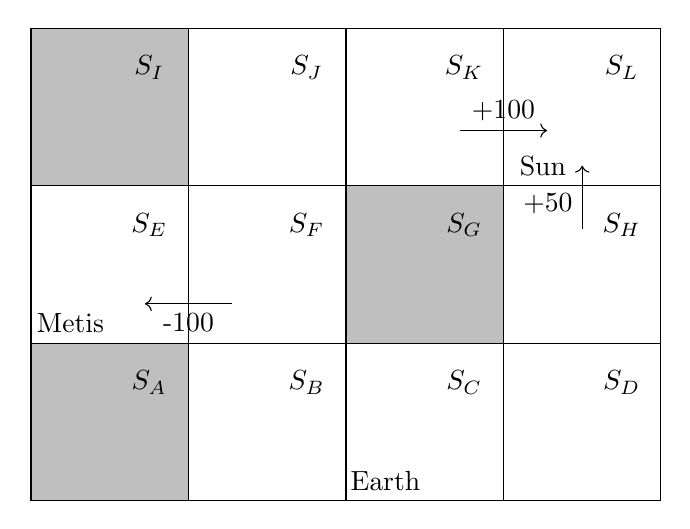
\begin{tikzpicture}
\draw[step=2cm] (0,0) grid (8, 6);

\node at (4.5, 0.25) {Earth};
\node at (6.5, 4.25) {Sun};
\node at (0.5, 2.25) {Metis};

\foreach \x/\y in {
    2/1, 0/2, 0/0} ]
    \draw[fill=white!50!gray] 
    (2*\x,2*\y) rectangle (2*\x + 2, 2*\y + 2);


\foreach \x/\y/\m in {
    0/2/I, 1/2/J, 2/2/K, 3/2/L,
    0/1/E, 1/1/F, 2/1/G, 3/1/H,
    0/0/A, 1/0/B, 2/0/C, 3/0/D}
    \node at (2*\x + 1.5,2*\y + 1.5) {$S_\m$};

\node[state, draw=none] (n1) at (5, 4.7) {};
\node[state, draw=none] (n2) at (7, 4.7) {};
\node[state, draw=none] (n3) at (7, 3) {};
\node[state, draw=none] (n4) at (1, 2.5) {};
\node[state, draw=none] (n5) at (3, 2.5) {};

\draw [->] (n1) to node[pos=0.5, above] { +100} (n2);
\draw [->] (n3) to node[pos=0.4, left] {+50} (n2);
\draw [->] (n5) to node[pos=0.5, below] {-100} (n4);

\end{tikzpicture}
\end{center}

Here are the details:

\begin{enumerate}
    \item Each grid cell is a state $S_A, S_B,..., S_L$ corresponding to a position in the solar system.
    \item The action space includes movement \texttt{up}/\texttt{down}/\texttt{left}/\texttt{right}. Transitions are \textbf{non-deterministic}. With probability $80\%$ the agent transitions to the intended state. With probability $10\%$ the agent slips left \emph{of the intended direction}. With probability $10\%$ the agent slips right \emph{of the intended direction}. For example, if the agent is in state $S_F$ and takes action \texttt{left},  it moves to state $S_E$ with 80\% probability, it moves to state $S_B$ (left of the intended direction) with 10\% probability, and it moves to state $S_J$ (right of the intended direction)  with 10\% probability,.
    \item It is not possible to move into blocked states, which are shaded grey, since they contain other planets. If the agent's action would move them out of bounds of the board or a blocked state, it remains in the same state.
    \item The start state is $S_C$ (Earth). The terminal states include both the $S_L$ (Sun) and $S_E$ (asteroid Metis).
    \item Non-zero rewards are depicted with arrows.  Flying into the Sun from the left gives positive reward $R(S_K, \texttt{a}, S_L) = +100$ $\forall \texttt{a} \in$ $\{\texttt{up},\texttt{down},\texttt{left},\texttt{right}\}$, since it is more fuel-efficient than flying into the sun from below (the agent can use the gravitational field of the planets in $S_A$ and $S_I$ in addition to $S_G$). However, approaching the Sun from the left has its risks, as flying into Metis is inadvisable and gives negative reward $R(S_F, \texttt{a}, S_E) = -100$ $\forall \texttt{a} \in$ $\{\texttt{up},\texttt{down},\texttt{left},\texttt{right}\}$. Note that flying into the Sun from below still achieves the goal and gives positive reward $R(S_H, \texttt{a}, S_L) = +50$ $\forall \texttt{a} \in$ $\{\texttt{up},\texttt{down},\texttt{left},\texttt{right}\}$. All other rewards are zero. 
\end{enumerate}

    
Below, let $V^*(s)$ denote the value function for state $s$ using the optimal policy $\pi^*(s)$.

\subsectionquestion{Synchronous Value Iteration}

\begin{parts}

    \part[3] Report the value of each state after a single round of \textbf{synchronous} value iteration in the table below. Initialize the value table $V^0(s) = 0$, $\forall s \in \{S_A \hdots S_L\}$ and assume $\gamma=0.9$. Visit each state in \textit{reverse alphabetical order}. Ignore the blocked states. Round your \textit{answers only} to the first decimal place. \textbf{Do not round intermediate values when calculating your answers.}
    
    \begin{center}
    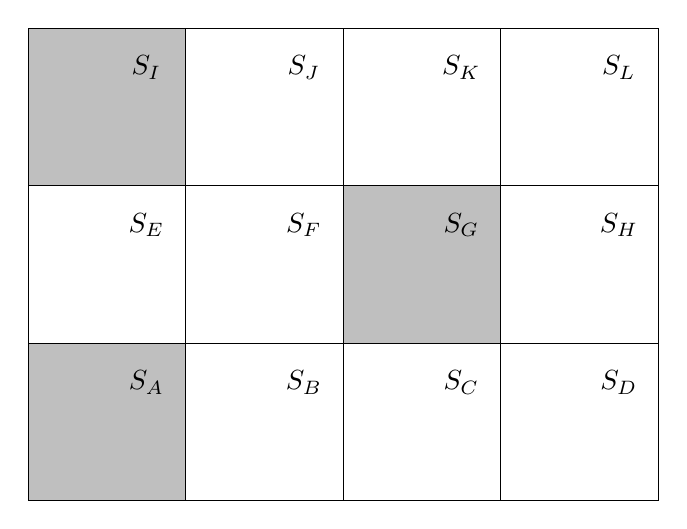
\begin{tikzpicture}
    \draw[step=2cm] (0,0) grid (8, 6);
    
    \foreach \x/\y in {
        2/1, 0/2, 0/0}
        \draw[fill=white!50!gray] 
        (2*\x,2*\y) rectangle (2*\x + 2, 2*\y + 2);
    
    
    \foreach \x/\y/\m in {
        0/2/I, 1/2/J, 2/2/K, 3/2/L,
        0/1/E, 1/1/F, 2/1/G, 3/1/H,
        0/0/A, 1/0/B, 2/0/C, 3/0/D}
        \node at (2*\x + 1.5,2*\y + 1.5) {$S_\m$};
        
    % WRITE YOUR SOLUTION HERE
    % Be careful NOT TO DELETE THE COMMA!
    % There MUST be a comma at the end of every line
    \foreach \x/\y/\m in {
        1/0/{}, % REPLACE THE {} WITH THE VALUE FOR STATE B HERE 
        2/0/{}, % REPLACE THE {} WITH THE VALUE FOR STATE C HERE 
        3/0/{}, % REPLACE THE {} WITH THE VALUE FOR STATE D HERE
        0/1/{}, % REPLACE THE {} WITH THE VALUE FOR STATE E HERE 
        1/1/{}, % REPLACE THE {} WITH THE VALUE FOR STATE F HERE
        3/1/{}, % REPLACE THE {} WITH THE VALUE FOR STATE H HERE 
        1/2/{}, % REPLACE THE {} WITH THE VALUE FOR STATE J HERE 
        2/2/{}, % REPLACE THE {} WITH THE VALUE FOR STATE K HERE 
        3/2/{}, % REPLACE THE {} WITH THE VALUE FOR STATE L HERE
        }  
        \node at (2*\x + 1,2*\y + 1) {$\m$};
    
    \end{tikzpicture}
    \end{center}
    
    
    \part[3] What is the policy, $\pi(s)$, that corresponds to the value table you calculated above? Write one of \texttt{up}, \texttt{down}, \texttt{left}, or \texttt{right} for each state. If multiple actions are acceptable, choose the one that comes alphabetically first. For terminal states, write \texttt{terminal}. Ignore the blocked states.
    
    \begin{center}
    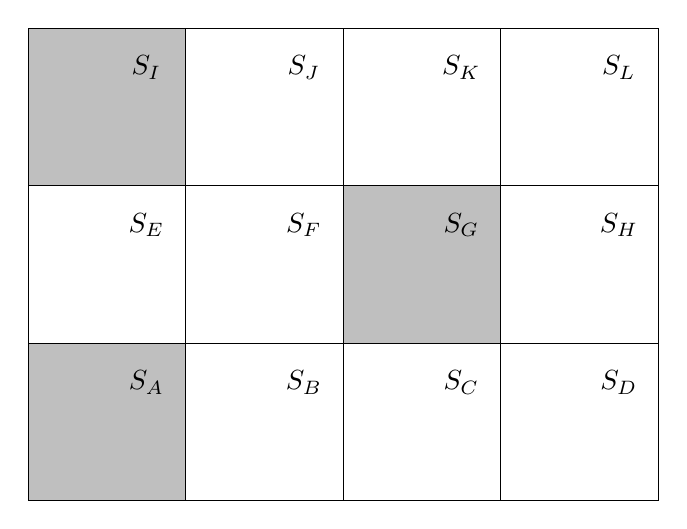
\begin{tikzpicture}
    \draw[step=2cm] (0,0) grid (8, 6);
    
    \foreach \x/\y in {
        2/1, 0/2, 0/0}
        \draw[fill=white!50!gray] 
        (2*\x,2*\y) rectangle (2*\x + 2, 2*\y + 2);
    
    
    \foreach \x/\y/\m in {
        0/2/I, 1/2/J, 2/2/K, 3/2/L,
        0/1/E, 1/1/F, 2/1/G, 3/1/H,
        0/0/A, 1/0/B, 2/0/C, 3/0/D}
        \node at (2*\x + 1.5,2*\y + 1.5) {$S_\m$};
    
    % WRITE YOUR SOLUTION HERE
    % Be careful NOT TO DELETE THE COMMA!
    % There MUST be a comma at the end of every line
    % You only have to write up, down, left, or right.
    % No need to write \texttt{up}
    \foreach \x/\y/\m in {
        1/0/{}, % REPLACE THE {} WITH THE POLICY FOR STATE B HERE 
        2/0/{}, % REPLACE THE {} WITH THE POLICY FOR STATE C HERE 
        3/0/{}, % REPLACE THE {} WITH THE POLICY FOR STATE D HERE
        0/1/{}, % REPLACE THE {} WITH THE POLICY FOR STATE E HERE 
        1/1/{}, % REPLACE THE {} WITH THE POLICY FOR STATE F HERE
        3/1/{}, % REPLACE THE {} WITH THE POLICY FOR STATE H HERE
        1/2/{}, % REPLACE THE {} WITH THE POLICY FOR STATE J HERE 
        2/2/{}, % REPLACE THE {} WITH THE POLICY FOR STATE K HERE 
        3/2/{}, % REPLACE THE {} WITH THE POLICY FOR STATE L HERE
        }  
        \node at (2*\x + 1,2*\y + 1) {\texttt{\m}};
    
    \end{tikzpicture}
    \end{center}
    
    
\end{parts}

\clearpage

\subsectionquestion{Asynchronous Value Iteration}

\begin{parts}
    
    \part[3] Starting over, report the value of each state for a single round of \textbf{asynchronous} value iteration in the table below.  Initialize the value table $V^0(s) = 0$, $\forall s \in \{S_A \hdots S_L\}$ and assume $\gamma=0.9$. Visit each state in \textit{reverse alphabetical order}. Ignore the blocked states. Round your \textit{answers only} to the first decimal place. \textbf{Do not round intermediate values when calculating your answers.}
    
    \begin{center}
    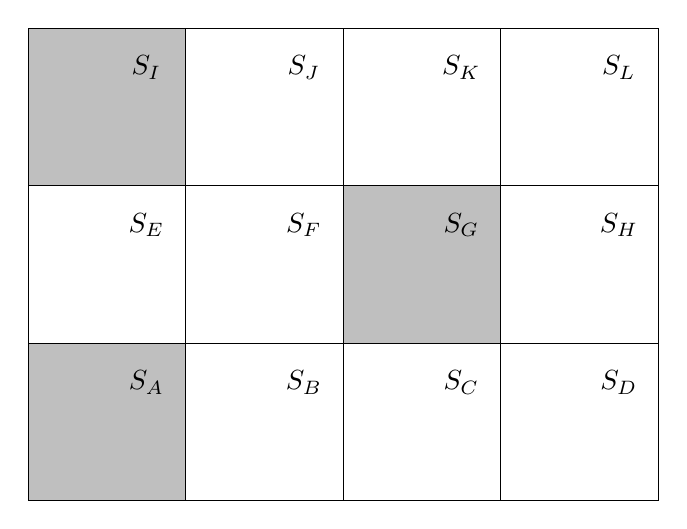
\begin{tikzpicture}
    \draw[step=2cm] (0,0) grid (8, 6);
    
    \foreach \x/\y in {
        2/1, 0/2, 0/0}
        \draw[fill=white!50!gray] 
        (2*\x,2*\y) rectangle (2*\x + 2, 2*\y + 2);
    
    
    \foreach \x/\y/\m in {
        0/2/I, 1/2/J, 2/2/K, 3/2/L,
        0/1/E, 1/1/F, 2/1/G, 3/1/H,
        0/0/A, 1/0/B, 2/0/C, 3/0/D}
        \node at (2*\x + 1.5,2*\y + 1.5) {$S_\m$};
        
    % WRITE YOUR SOLUTION HERE
    % Be careful NOT TO DELETE THE COMMA!
    % There MUST be a comma at the end of every line
    \foreach \x/\y/\m in {
        1/0/{}, % REPLACE THE {} WITH THE VALUE FOR STATE B HERE 
        2/0/{}, % REPLACE THE {} WITH THE VALUE FOR STATE C HERE 
        3/0/{}, % REPLACE THE {} WITH THE VALUE FOR STATE D HERE
        0/1/{}, % REPLACE THE {} WITH THE VALUE FOR STATE E HERE 
        1/1/{}, % REPLACE THE {} WITH THE VALUE FOR STATE F HERE
        3/1/{}, % REPLACE THE {} WITH THE VALUE FOR STATE H HERE 
        1/2/{}, % REPLACE THE {} WITH THE VALUE FOR STATE J HERE 
        2/2/{}, % REPLACE THE {} WITH THE VALUE FOR STATE K HERE 
        3/2/{}, % REPLACE THE {} WITH THE VALUE FOR STATE L HERE
        }  
        \node at (2*\x + 1,2*\y + 1) {$\m$};
    
    \end{tikzpicture}
    \end{center}
    
    
    \part[3] What is the policy, $\pi(s)$, that corresponds to the value table you calculated above? Write one of \texttt{up}, \texttt{down}, \texttt{left}, or \texttt{right} for each state. If multiple actions are acceptable, choose the one that comes alphabetically first. For terminal states, write \texttt{terminal}. Ignore the blocked states.
    
    \begin{center}
    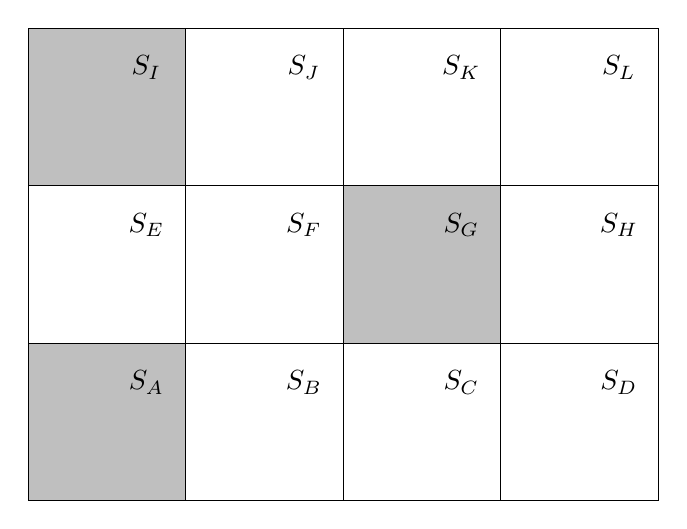
\begin{tikzpicture}
    \draw[step=2cm] (0,0) grid (8, 6);
    
    \foreach \x/\y in {
        2/1, 0/2, 0/0}
        \draw[fill=white!50!gray] 
        (2*\x,2*\y) rectangle (2*\x + 2, 2*\y + 2);
    
    
    \foreach \x/\y/\m in {
        0/2/I, 1/2/J, 2/2/K, 3/2/L,
        0/1/E, 1/1/F, 2/1/G, 3/1/H,
        0/0/A, 1/0/B, 2/0/C, 3/0/D}
        \node at (2*\x + 1.5,2*\y + 1.5) {$S_\m$};
    
    % WRITE YOUR SOLUTION HERE
    % Be careful NOT TO DELETE THE COMMA!
    % There MUST be a comma at the end of every line
    % You only have to write up, down, left, or right.
    % No need to write \texttt{up}
    \foreach \x/\y/\m in {
        1/0/{}, % REPLACE THE {} WITH THE POLICY FOR STATE B HERE 
        2/0/{}, % REPLACE THE {} WITH THE POLICY FOR STATE C HERE 
        3/0/{}, % REPLACE THE {} WITH THE POLICY FOR STATE D HERE
        0/1/{}, % REPLACE THE {} WITH THE POLICY FOR STATE E HERE 
        1/1/{}, % REPLACE THE {} WITH THE POLICY FOR STATE F HERE
        3/1/{}, % REPLACE THE {} WITH THE POLICY FOR STATE H HERE
        1/2/{}, % REPLACE THE {} WITH THE POLICY FOR STATE J HERE 
        2/2/{}, % REPLACE THE {} WITH THE POLICY FOR STATE K HERE 
        3/2/{}, % REPLACE THE {} WITH THE POLICY FOR STATE L HERE
        }  
        \node at (2*\x + 1,2*\y + 1) {\texttt{\m}};
    
    \end{tikzpicture}
    \end{center}
    
    
    \clearpage
    
    \part[3] Below, we give you the value of each state one round before the convergence of \textbf{asynchronous} value iteration.\footnote{This is actually one round before the \emph{policy} convergence, not the \emph{value} convergence. The values we provide are the values after the third iteration.} What is the final value of each state, $V^*(s)$? Be sure to use \textbf{asynchronous} value iteration, and visit each state in \textit{reverse alphabetical order}. Ignore the blocked states. Round your \textit{answers only} to the first decimal place. \textbf{Do not round intermediate values when calculating your answers.}
    
    \begin{center}
    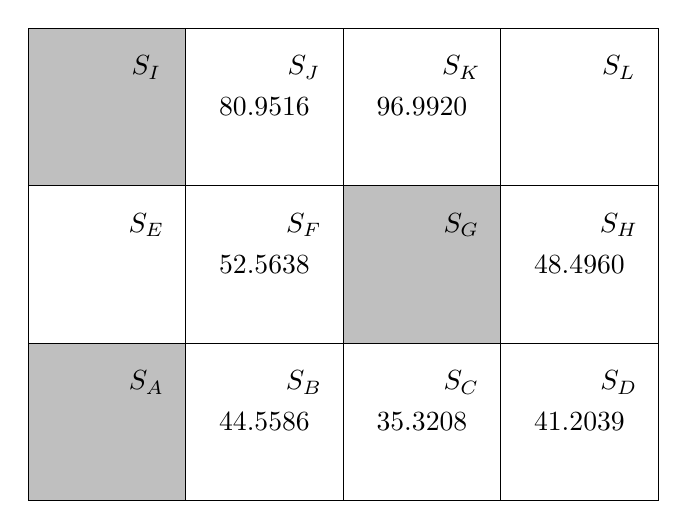
\begin{tikzpicture}
    \draw[step=2cm] (0,0) grid (8, 6);
    
    \foreach \x/\y in {
        2/1, 0/2, 0/0}
        \draw[fill=white!50!gray] 
        (2*\x,2*\y) rectangle (2*\x + 2, 2*\y + 2);
    
    
    \foreach \x/\y/\m in {
        0/2/I, 1/2/J, 2/2/K, 3/2/L,
        0/1/E, 1/1/F, 2/1/G, 3/1/H,
        0/0/A, 1/0/B, 2/0/C, 3/0/D}
        \node at (2*\x + 1.5,2*\y + 1.5) {$S_\m$};
    
    % VALUES ONE ROUND BEFORE CONVERGENCE   
    \foreach \x/\y/\m in {
        1/0/{44.5586}, % B
        2/0/{35.3208}, % C
        3/0/{41.2039}, % D
        0/1/{},  % E (terminal state, so no need to store value)
        1/1/{52.5638}, % F
        3/1/{48.4960}, % H
        1/2/{80.9516}, % J
        2/2/{96.9920}, % K
        3/2/{},  % L
        }  
        \node at (2*\x + 1,2*\y + 1) {$\m$};
    
    \end{tikzpicture}
    \end{center}
    
    \textbf{Your solution:}
    
    \begin{center}
    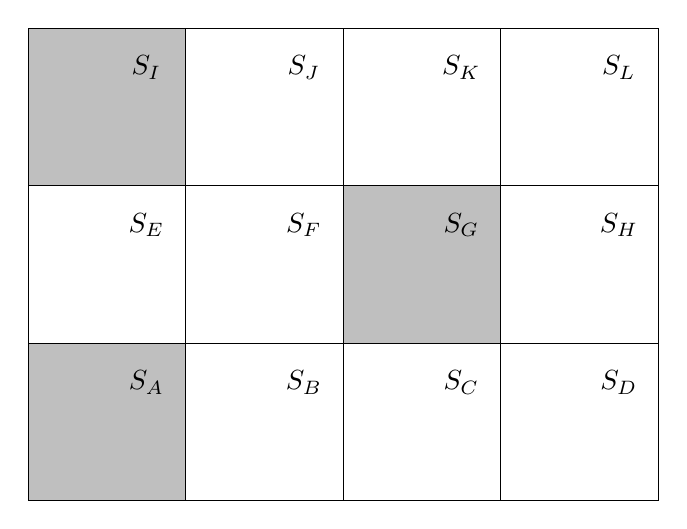
\begin{tikzpicture}
    \draw[step=2cm] (0,0) grid (8, 6);
    
    \foreach \x/\y in {
        2/1, 0/2, 0/0}
        \draw[fill=white!50!gray] 
        (2*\x,2*\y) rectangle (2*\x + 2, 2*\y + 2);
    
    
    \foreach \x/\y/\m in {
        0/2/I, 1/2/J, 2/2/K, 3/2/L,
        0/1/E, 1/1/F, 2/1/G, 3/1/H,
        0/0/A, 1/0/B, 2/0/C, 3/0/D}
        \node at (2*\x + 1.5,2*\y + 1.5) {$S_\m$};
        
    % WRITE YOUR SOLUTION HERE
    % Be careful NOT TO DELETE THE COMMA!
    % There MUST be a comma at the end of every line
    \foreach \x/\y/\m in {
        1/0/{}, % REPLACE THE {} WITH THE VALUE FOR STATE B HERE 
        2/0/{}, % REPLACE THE {} WITH THE VALUE FOR STATE C HERE 
        3/0/{}, % REPLACE THE {} WITH THE VALUE FOR STATE D HERE
        0/1/{}, % REPLACE THE {} WITH THE VALUE FOR STATE E HERE 
        1/1/{}, % REPLACE THE {} WITH THE VALUE FOR STATE F HERE
        3/1/{}, % REPLACE THE {} WITH THE VALUE FOR STATE H HERE
        1/2/{}, % REPLACE THE {} WITH THE VALUE FOR STATE J HERE 
        2/2/{}, % REPLACE THE {} WITH THE VALUE FOR STATE K HERE 
        3/2/{}, % REPLACE THE {} WITH THE VALUE FOR STATE L HERE
        } 
        \node at (2*\x + 1,2*\y + 1) {\texttt{\m}};
    
    \end{tikzpicture}
    \end{center}
    
    
    \clearpage
    
    \part[3] What is the policy, $\pi^*(s)$, that corresponds to $V^*(s)$? Write one of \texttt{up}, \texttt{down}, \texttt{left}, or \texttt{right} for each state. If multiple actions are acceptable, choose the one that comes alphabetically first. For terminal states, write \texttt{terminal}. Ignore the blocked states.
    
    \begin{center}
    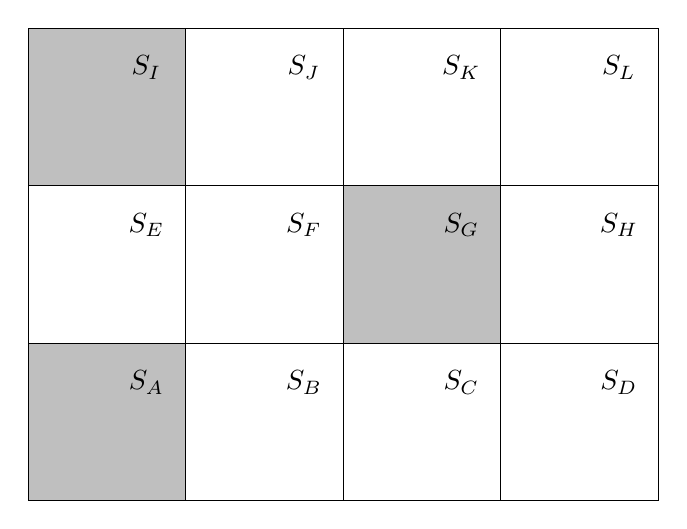
\begin{tikzpicture}
    \draw[step=2cm] (0,0) grid (8, 6);
    
    \foreach \x/\y in {
        2/1, 0/2, 0/0}
        \draw[fill=white!50!gray] 
        (2*\x,2*\y) rectangle (2*\x + 2, 2*\y + 2);
    
    
    \foreach \x/\y/\m in {
        0/2/I, 1/2/J, 2/2/K, 3/2/L,
        0/1/E, 1/1/F, 2/1/G, 3/1/H,
        0/0/A, 1/0/B, 2/0/C, 3/0/D}
        \node at (2*\x + 1.5,2*\y + 1.5) {$S_\m$};
    
    % WRITE YOUR SOLUTION HERE
    % Be careful NOT TO DELETE THE COMMA!
    % There MUST be a comma at the end of every line
    % You only have to write up, down, left, or right.
    % No need to write \texttt{up}
    \foreach \x/\y/\m in {
        1/0/{}, % REPLACE THE {} WITH THE POLICY FOR STATE B HERE 
        2/0/{}, % REPLACE THE {} WITH THE POLICY FOR STATE C HERE 
        3/0/{}, % REPLACE THE {} WITH THE POLICY FOR STATE D HERE
        0/1/{}, % REPLACE THE {} WITH THE POLICY FOR STATE E HERE 
        1/1/{}, % REPLACE THE {} WITH THE POLICY FOR STATE F HERE
        3/1/{}, % REPLACE THE {} WITH THE POLICY FOR STATE H HERE
        1/2/{}, % REPLACE THE {} WITH THE POLICY FOR STATE J HERE 
        2/2/{}, % REPLACE THE {} WITH THE POLICY FOR STATE K HERE 
        3/2/{}, % REPLACE THE {} WITH THE POLICY FOR STATE L HERE
        } 
        \node at (2*\x + 1,2*\y + 1) {\texttt{\m}};
    
    \end{tikzpicture}
    \end{center}
    

\end{parts}

\clearpage

\sectionquestion{Q-Learning}

Let's consider the same grid world as before:

\begin{center}
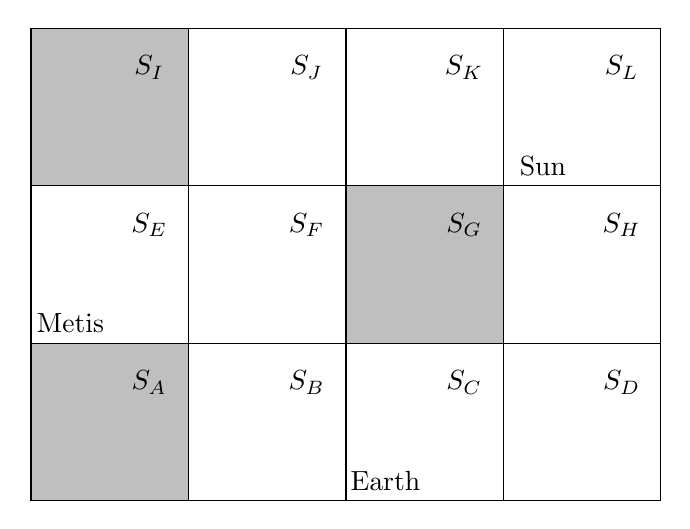
\begin{tikzpicture}
\draw[step=2cm] (0,0) grid (8, 6);

\node at (4.5, 0.25) {Earth};
\node at (6.5, 4.25) {Sun};
\node at (0.5, 2.25) {Metis};

\foreach \x/\y in {
    2/1, 0/2, 0/0}
    \draw[fill=white!50!gray] 
    (2*\x,2*\y) rectangle (2*\x + 2, 2*\y + 2);


\foreach \x/\y/\m in {
    0/2/I, 1/2/J, 2/2/K, 3/2/L,
    0/1/E, 1/1/F, 2/1/G, 3/1/H,
    0/0/A, 1/0/B, 2/0/C, 3/0/D}
    \node at (2*\x + 1.5,2*\y + 1.5) {$S_\m$};

\end{tikzpicture}
\end{center}

This time, however, suppose we \textbf{don't know} the reward function or the transition probability between states. Some rules for this setup are:

\begin{enumerate}
    \item Each grid cell is a state $S_A, S_B, \hdots , S_L$ corresponding to a position in the solar system.
    \item The action space of the agent is: $\{\texttt{up}, \texttt{down}, \texttt{left}, \texttt{right}\}$.
    \item If the agent hits the edge of the board, it remains in the same state. It is not possible to move into blocked states, which are shaded grey, since they contain other planets.
    \item The start state is $S_C$ (Earth). The terminal states include both the $S_L$ (Sun) and $S_E$ (asteroid Metis).
    \item Use the discount factor $\gamma = 0.9$, $\epsilon=0.5$, and learning rate $\alpha=0.1$.
\end{enumerate}

We will go through three iterations of Q-learning in this section. Initialize $Q(s,a)=0$, $\forall s \in \{S_A, \hdots, S_L\}$, $\forall a \in \{\texttt{up}, \texttt{down}, \texttt{left}, \texttt{right}\}$. 

\begin{parts}
\part[1] \sall If the agent were to act greedily, what action would it take at this time?

{
\checkboxchar{$\Box$} \checkedchar{$\blacksquare$}
\begin{checkboxes}
    % Change \choice to \CorrectChoice
    \choice \texttt{up}
    \choice \texttt{down}
    \choice \texttt{left}
    \choice \texttt{right}
\end{checkboxes}
}


\part[1] Beginning at state $S_C$, you take the action \texttt{right} and receive a reward of 0. You are now in state $S_D$. What is the new value for $Q(S_C, \texttt{right})$, assuming the update for deterministic transitions? Round your answer to the fourth decimal place.

\begin{your_solution}[title={$Q(S_C, \texttt{right})$},height=2cm,width=4cm]
    % YOUR ANSWER
\end{your_solution}

\clearpage

\part[1] What is the new value for $Q(S_C, \texttt{right})$, using the temporal difference error update? Round your answer to the fourth decimal place.

\begin{your_solution}[title={$Q(S_C, \texttt{right})$},height=2cm,width=4cm]
    % YOUR ANSWER
\end{your_solution}

\part[1] \sall Continue to update your Q-function (as calculated by the temporal difference error update) from above. This time, though, assume your run has brought you to state $S_H$ with no updates to the Q-function in the process. If the agent were to act greedily, what action would it take at this time?

{
\checkboxchar{$\Box$} \checkedchar{$\blacksquare$}
\begin{checkboxes}
    % Change \choice to \CorrectChoice
    \choice \texttt{up}
    \choice \texttt{down}
    \choice \texttt{left}
    \choice \texttt{right}
\end{checkboxes}
}


\part[1] Beginning at state $S_H$, you take the action \texttt{up}, receive a reward of +50, and the run terminates. What is the new value for $Q(S_H, \texttt{up})$, assuming the update for deterministic transitions? Round your answer to the fourth decimal place.

\begin{your_solution}[title={$Q(S_H, \texttt{up})$},height=2cm,width=4cm]
    % YOUR ANSWER
\end{your_solution}

\part[1] What is the new value for $Q(S_H, \texttt{up})$, using the temporal difference error update? Round your answer to the fourth decimal place.

\begin{your_solution}[title={$Q(S_H, \texttt{up})$},height=2cm,width=4cm]
    % YOUR ANSWER
\end{your_solution}

\part[1] \sall Continue to update your Q-function (as calculated by the temporal difference error update) from above. You start from state $S_C$ since the previous run terminated, but manage to make it to state $S_F$ with no updates to the Q-function. If the agent were to act greedily, what action would it take at this time?

{
\checkboxchar{$\Box$} \checkedchar{$\blacksquare$}
\begin{checkboxes}
    % Change \choice to \CorrectChoice
    \choice \texttt{up}
    \choice \texttt{down}
    \choice \texttt{left}
    \choice \texttt{right}
\end{checkboxes}
}


\clearpage

\part[1] Beginning at state $S_F$, you take the action \texttt{left}, receive a reward of -100, and the run terminates. What is the new value for $Q(S_F, \texttt{left})$, assuming the update for deterministic transitions? Round your answer to the fourth decimal place.

\begin{your_solution}[title={$Q(S_F, \texttt{left})$},height=2cm,width=4cm]
    % YOUR ANSWER
\end{your_solution}

\part[1] What is the new value for $Q(S_F, \texttt{left})$, using the temporal difference error update? Round your answer to the fourth decimal place.

\begin{your_solution}[title={$Q(S_F, \texttt{left})$},height=2cm,width=4cm]
    % YOUR ANSWER
\end{your_solution}

\end{parts}

\clearpage

\sectionquestion{Function Approximation}
\label{sec:FA}

In this question we will motivate function approximation for solving Markov Decision Processes by looking at Breakout, a game on the Atari 2600. The Atari 2600 is a gaming system released in the 1980s, but nevertheless is a popular target for reinforcement learning papers and benchmarks. The Atari 2600 has a resolution of $160 \times 192$ pixels. In the case of Breakout, we try to move the paddle to hit the ball in order to break as many tiles above as possible. We have the following actions:
\begin{itemize}
    \item Move the paddle left
    \item Move the paddle right
    \item Do nothing
\end{itemize}

\begin{figure}[H]
    \centering
    \begin{subfigure}{0.5\textwidth}
        
\includegraphics[width=0.99\linewidth]{atari_crop_color.png}
        \caption{Atari Breakout}
        \label{fig:breakout}
    \end{subfigure}%
    \begin{subfigure}{0.5\textwidth}
        
\includegraphics[width=0.99\linewidth]{atari_crop_bw.png}
        \caption{Black and white Breakout}
        \label{fig:bw_breakout}
    \end{subfigure}
    \caption{Atari Breakout. \ref{fig:breakout} is what Breakout looks like. We have the paddle in the bottom of the screen aiming to hit the ball in order to break the tiles at the top of the screen. \ref{fig:bw_breakout} is our transformation of Atari Breakout into black and white pixels for the purpose of some of the following problems.}
    \label{fig:my_label}
\end{figure}

\begin{parts}
    \part[1] Suppose we are dealing with the black and white version of Breakout\footnote{Play a ``Google''-Doodle version \href{https://elgoog.im/breakout/}{here}} as in Figure~\ref{fig:bw_breakout}. Furthermore, suppose we are representing the state of the game as just a vector of pixel values without considering if a certain pixel is always black or white. Since we are dealing with the black and white version of the game, these pixel values can either be 0 or 1.
    
    What is the size of the state space? \\
    \begin{your_solution}[title = Answer, height=2cm,width=3cm]
        % YOUR ANSWER 
    \end{your_solution}
    
    
    \part[1] In the same setting as the previous part, suppose we wish to apply Q-learning to this problem. What is the size of the Q-value table we will need?\\
    \begin{your_solution}[title =Answer, height=2cm,width=3cm]
        % YOUR ANSWER 
    \end{your_solution}\\
    
    
    
    \part[1] Now assume we are dealing with the colored version of Breakout as in Figure~\ref{fig:breakout}. Now each pixel is a tuple of real valued numbers between $0$ and $1$. For example, black is represented as $(0, 0, 0)$ and white is $(1, 1, 1)$. 
    
    What is the size of the state space and Q-value table we will need?
    \\
    \begin{your_solution}[title=Answer,height=2cm]
        % YOUR ANSWER 
    \end{your_solution}\\
    
    
    % break from here
    By now you should see that we will need a huge table in order to apply Q-learning (and similarly value iteration and policy iteration) to Breakout given this state representation. This table would not even fit in the memory of any reasonable computer! Now this choice of state representation is particularly na\"ive. If we choose a better state representation, we could drastically reduce the table size needed. 
    
    On the other hand, perhaps we don't want to spend our days feature engineering a state representation for Breakout. Instead we can apply function approximation to our reinforcement algorithms! The whole idea of function approximation is that states nearby to the state of interest should have \emph{similar} values. That is, we should be able to generalize the value of a state to nearby and unseen states.
    
    Let us define $q_\pi(s, a)$ as the true action value function of the current policy $\pi$. Assume $q_\pi(s,a)$ is given to us by some oracle. Also define $q(s, a; \wv)$ as the action value predicted by the function approximator parameterized by $\wv$. Here $\wv$ is a matrix of size $\dim(S) \times |\mathcal{A}|$, where $\dim(S)$ denotes the dimension of the state space. Clearly we want to have $q(s, a; \wv)$ be close to $q_\pi(s, a)$ for all $(s, a)$ pairs we see. This is just our standard regression setting. That is, our objective function is just the Mean Squared Error:
    \begin{align}
    J(\wv) = \frac{1}{2} \frac{1}{N} \sum_{s\in\mathcal{S}, a\in\mathcal{A}} \left(q_\pi(s, a) - q(s, a; \wv) \right)^2.
    \end{align}
    Because we want to update for each example stochastically\footnote{This is not really stochastic, you will be asked in a bit why.}, we get the following update rule:
    \begin{align}
    \wv \leftarrow \wv - \alpha \left(q(s, a; \wv) - q_\pi(s,a) \right) \nabla_\wv q(s, a; \wv).
    \end{align}
    
    However, more often than not we will not have access to the oracle that gives us our target $q_\pi(s, a)$. So how do we get the target to regress $q(s, a; \wv)$ on? One way is to bootstrap an estimate of the action value under a greedy policy using the function approximator itself. That is to say
    \begin{align}
    q_\pi (s, a) \approx r + \gamma \max_{a'} q(s', a'; \wv)
    \end{align}
    where $r$ is the reward observed from taking action $a$ at state $s$, $\gamma$ is the discount factor and $s'$ is the state resulting from taking action $a$ at state $s$. This target is often called the Temporal Difference (TD) target, and gives rise to the following update for the parameters of our function approximator in lieu of a tabular update:
    
    \begin{align}
    \wv \leftarrow \wv - \alpha \bigg( \underbrace{q(s, a; \wv) - \underbrace{\big (r + \gamma \max_{a'}q(s', a'; \wv)\big)}_{\text{TD Target}}}_{\text{TD Error}} \bigg) \nabla_\wv q(s, a; \wv).
    \end{align}
    
    \part[2] Consider the setting where we can represent our state by some vector $\sv$, action $a \in \{0, 1, 2\}$ and we choose a linear approximator. That is:
    \begin{align}
    \label{eq:linearEQ}
    q(\sv, a; \wv) = \sv^T\wv_a
    \end{align}
    Again, assume we are in the black and white setting of Breakout as in Figure~\ref{fig:bw_breakout}. Show that tabular Q-learning is just a special case of Q-learning with a linear function approximator by describing a construction of $\sv$. (\textbf{Hint}: Engineer features such that Eq. (\ref{eq:linearEQ}) encodes a table lookup)
    
    \begin{your_solution}[title=Answer,height=6cm]
        % YOUR ANSWER 
    \end{your_solution}
    
    \part[3] Stochastic Gradient Descent works because we can assume that the samples we receive are independent and identically distributed. Is that the case here? If not, why and what are some ways you think you could combat this issue?
    
    \begin{your_solution}[title=Answer,height=4cm]
        % YOUR ANSWER 
    \end{your_solution}
\end{parts}

\clearpage

\sectionquestion{Empirical Questions}

The following parts should be completed after you work through the programming portion of this assignment (Section \ref{sec:code}). 

\begin{parts}
    \part[4] Run Q-learning on the mountain car environment using both tile and raw features. 
    
    For the raw features: run for 2000 episodes with max iterations of 200, $\epsilon$ set to 0.05, $\gamma$ set to 0.999, and a learning rate of 0.001. 
    
    For the tile features: run for 400 episodes with max iterations of 200, $\epsilon$ set to 0.05, $\gamma$ set to 0.99, and a learning rate of 0.00005.
    
    For each set of features, plot the return (sum of all rewards in an episode) per episode on a line graph. On the same graph, also plot the rolling mean over a 25 episode window. Comment on the difference between the plots.
    
    \begin{your_solution}[title=Plot of Raw, height=10cm]
        % YOUR ANSWER 
        % Figure inclusion example:
        % \begin{center}
        %    \includegraphics[width=0.8\linewidth]{YOUR IMAGE FILE}
        % \end{center}
    \end{your_solution}
    
    \begin{your_solution}[title=Plot of Tile, height=10cm]
        % YOUR ANSWER
        % Figure inclusion example:
        % \begin{center}
        %    \includegraphics[width=0.8\linewidth]{YOUR IMAGE FILE}
        % \end{center}
    \end{your_solution}
    
    \begin{your_solution}[title=Comment,height=5cm]
        % YOUR ANSWER 
    \end{your_solution}
    \clearpage
    \begin{figure}[H]
        \centering
        \begin{subfigure}{0.5\textwidth}
            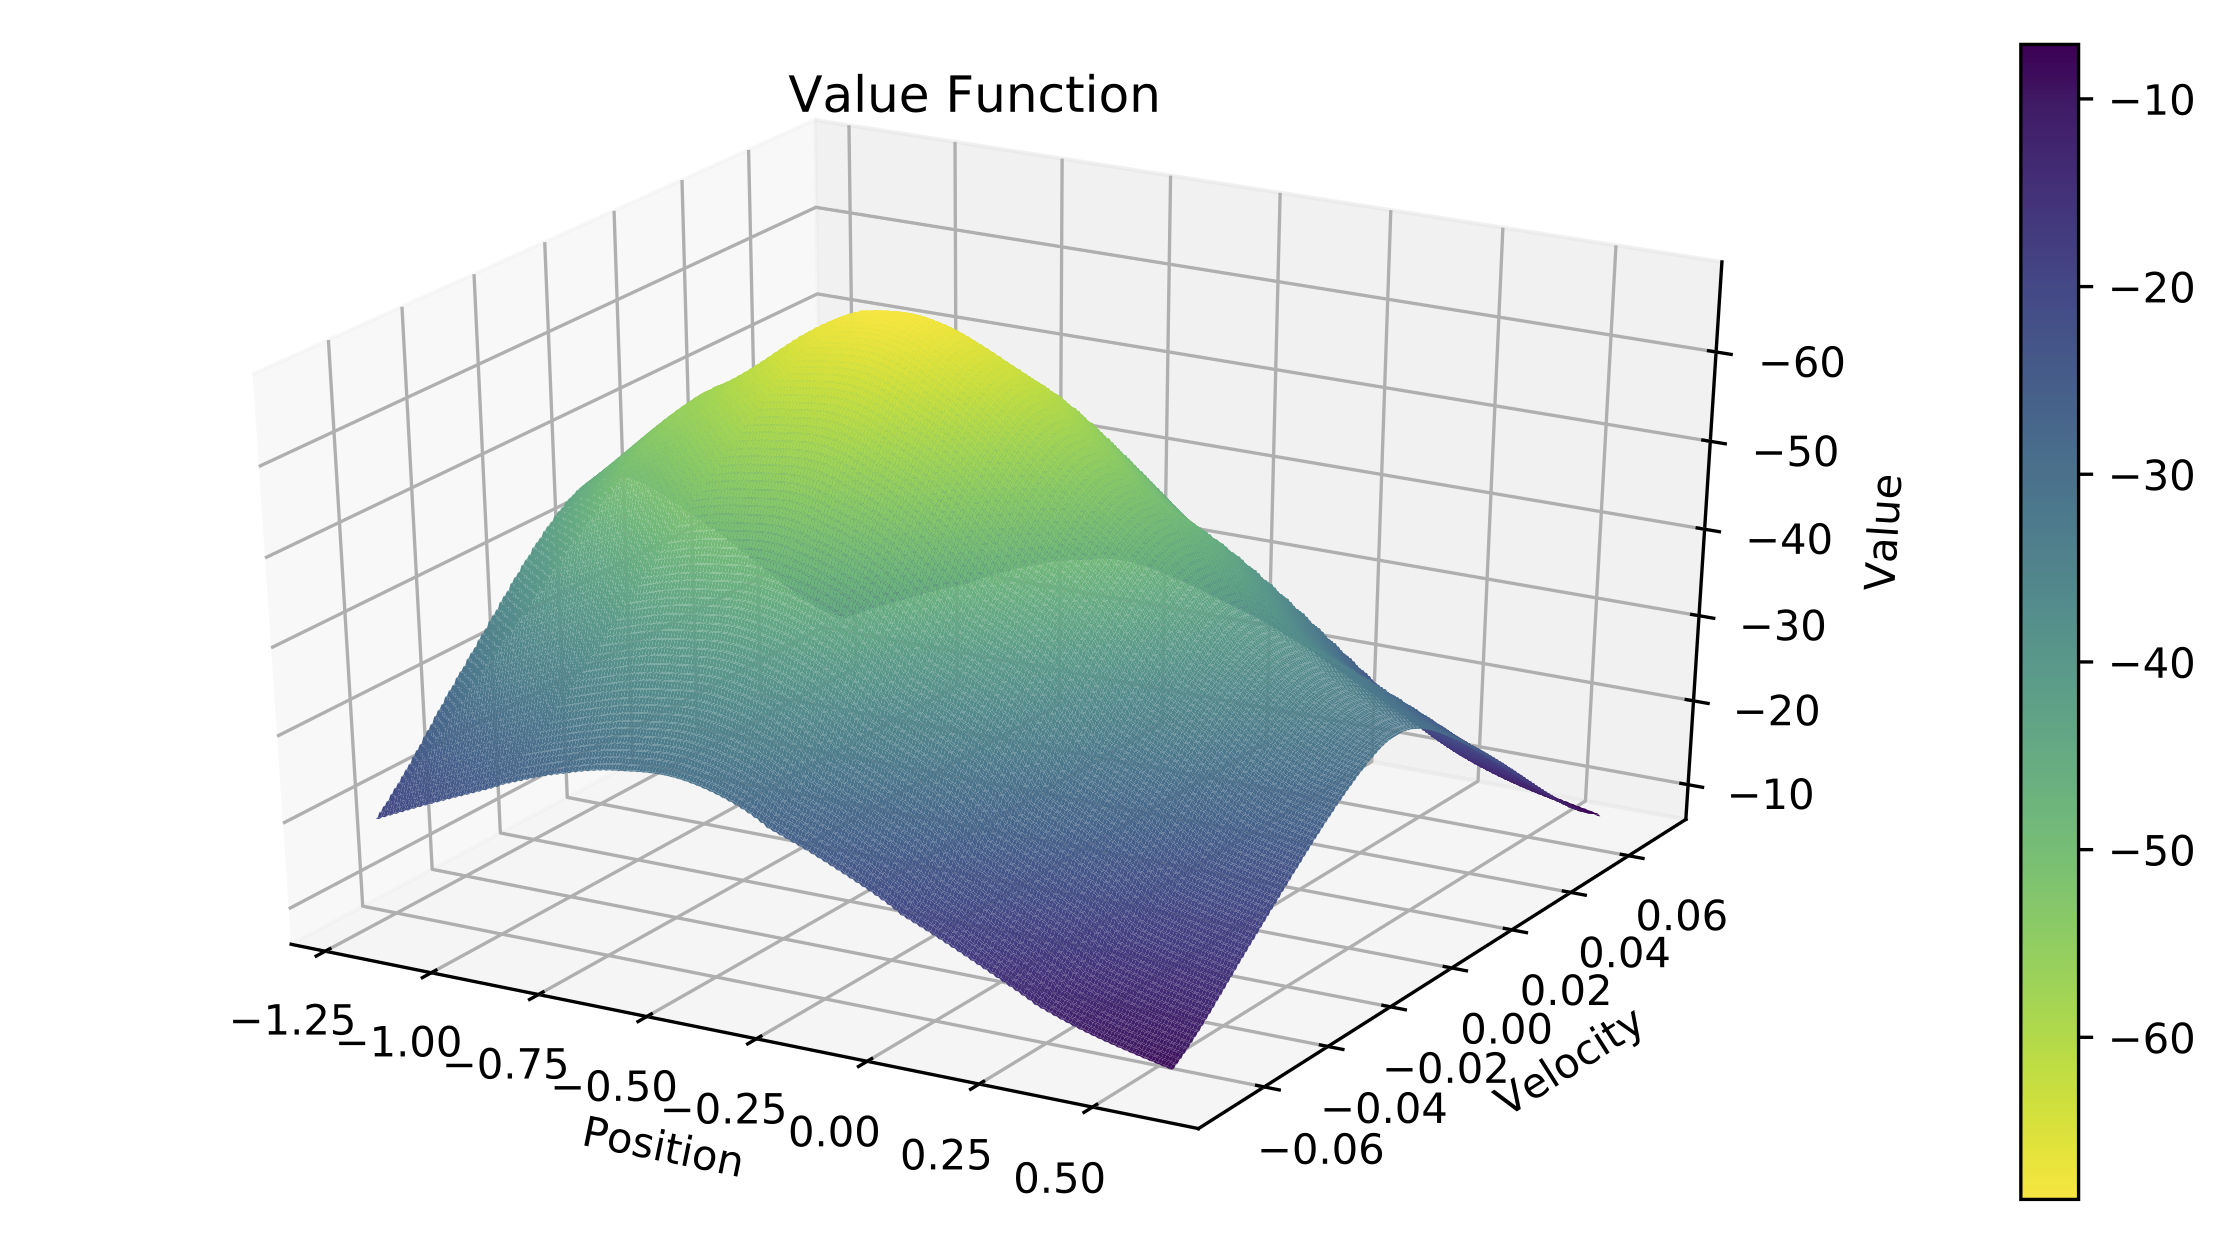
\includegraphics[width=\linewidth]{value_A.png}
            \caption{}
            \label{fig:value_a}
        \end{subfigure}%
        \begin{subfigure}{0.5\textwidth}
            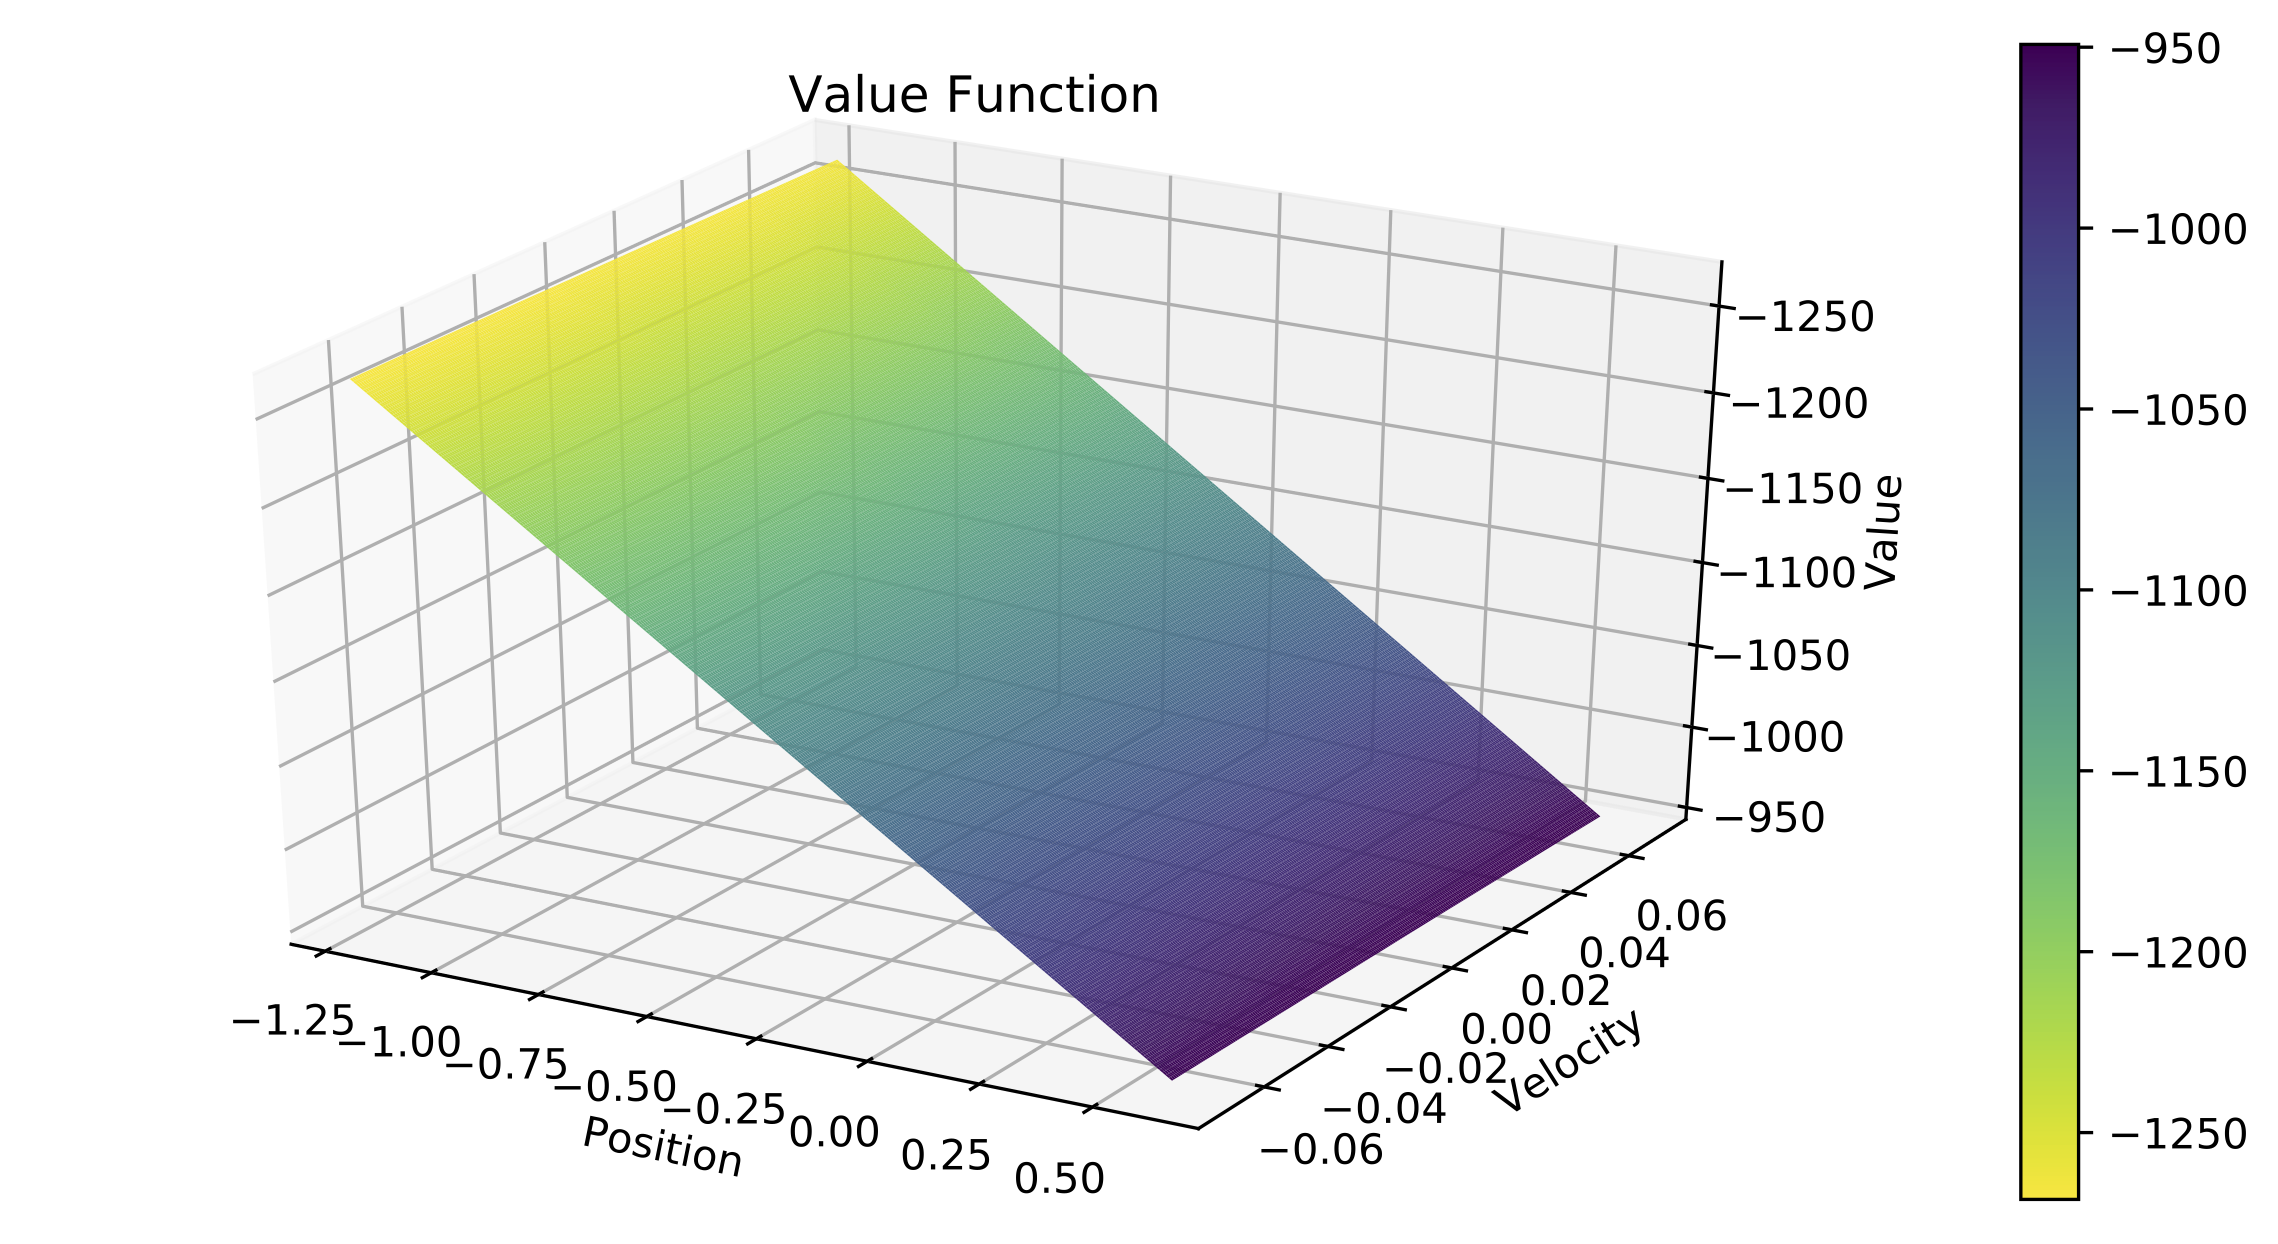
\includegraphics[width=\linewidth]{value_B.png}
            \caption{}
            \label{fig:value_b}
        \end{subfigure}
        \caption{Estimated optimal value function visualizations for both types of features}
        \label{fig:value}
    \end{figure}
    
    \part[2] For both raw and tile features, we have run Q-learning with some good parameters and created visualizations of the value functions after many episodes. For each plot in Figure~\ref{fig:value}, write down which features (raw or tile) were likely used in Q-learning with function approximation. Explain your reasoning. In addition, interpret each of these plots in the context of the mountain car environment.
    
    \begin{your_solution}[title=Answer,height=5cm]
        % YOUR ANSWER 
    \end{your_solution}


    \part[2] We see that Figure~\ref{fig:value_b} seems to look like a plane. Can the value function depicted in this plot ever be nonlinear (linear here \textit{strictly} refers to a function that can be expressed in the form of $y = \Av \xv + \bv$)? If so, describe a potential shape. If not, explain why.
    
    \textit{Hint:} How do we calculate the value of a state given the Q-values?

    \begin{your_solution}[title=Answer,height=5cm]
        % YOUR ANSWER 
    \end{your_solution}
    
    
        
    
    \begin{figure}[H]
        \centering
        \begin{subfigure}{0.5\textwidth}
            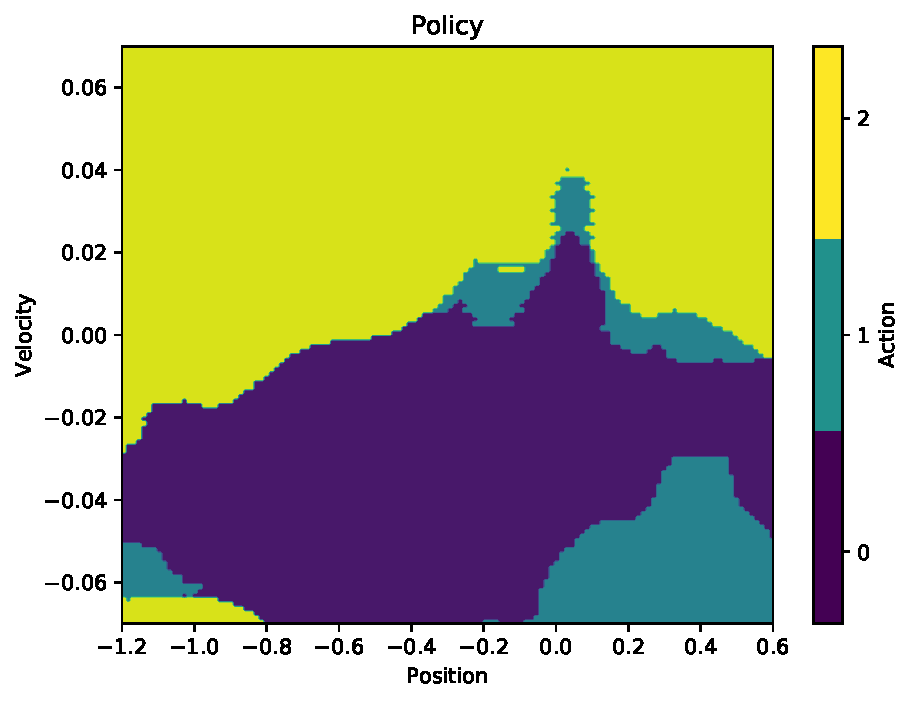
\includegraphics[width=\linewidth]{policy_A.pdf}
            \caption{}
            \label{fig:policy_a}
        \end{subfigure}%
        \begin{subfigure}{0.5\textwidth}
            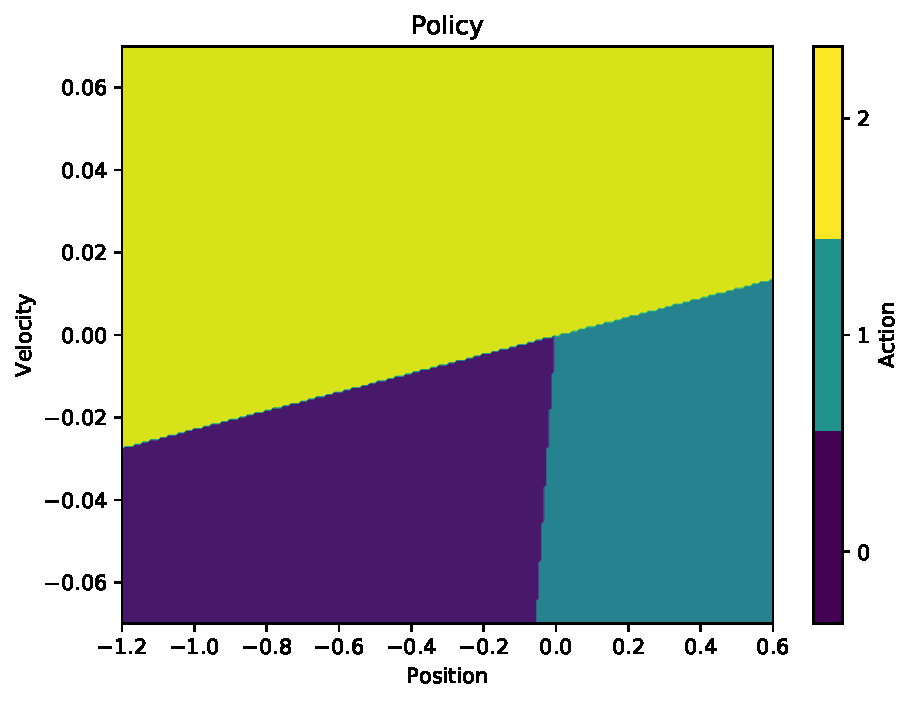
\includegraphics[width=\linewidth]{policy_B.pdf}
            \caption{}
            \label{fig:policy_b}
        \end{subfigure}
        \caption{Estimated optimal policy visualizations for both types of features}
        \label{fig:policy}
    \end{figure}

    \part[2] In a similar fashion to the previous question, we have created visualizations of the potential policies learned. For each plot in Figure~\ref{fig:policy}, write down which features (raw or tile) were likely used in Q-learning with function approximation. Explain your reasoning. In addition, interpret each of these plots in the context of the mountain car environment. Specifically, why are the edges linear v.s. non-linear? Why do they learn these patches at these specific locations? 
        
    \begin{your_solution}[title=Answer,height=5cm]
        % YOUR ANSWER 
    \end{your_solution}
\end{parts}

    \clearpage
    \end{questions}
\newpage
\section{Collaboration Questions}
After you have completed all other components of this assignment, report your answers to these questions regarding the collaboration policy. Details of the policy can be found \href{http://www.cs.cmu.edu/~mgormley/courses/10601/syllabus.html}{here}.
\begin{enumerate}
    \item Did you receive any help whatsoever from anyone in solving this assignment? If so, include full details.
    \item Did you give any help whatsoever to anyone in solving this assignment? If so, include full details.
    \item Did you find or come across code that implements any part of this assignment ? If so, include full details.
\end{enumerate}

\begin{your_solution}[height=6cm]
% YOUR ANSWER 

\end{your_solution}
\newpage
\section{Programming [68 Points]}
\label{sec:code}

Your goal in this assignment is to implement Q-learning with linear function approximation to solve the mountain car environment. You will implement all of the functions needed to initialize, train, evaluate, and obtain the optimal policies and action values with Q-learning. In this assignment we will provide the environment for you. The program you write will be automatically graded using the Gradescope system.

\subsection{Specification of Mountain Car}
In this assignment, you will be given code that fully defines the Mountain Car environment. In Mountain Car you control a car that starts at the bottom of a valley. Your goal is to reach the flag at the top right, as seen in Figure~\ref{fig:mountaincar}. However, your car is under-powered and cannot climb up the hill by itself. Instead you must learn to leverage gravity and momentum to make your way to the flag. It would also be good to get to this flag as fast as possible.

\begin{figure}[H]
    \centering
    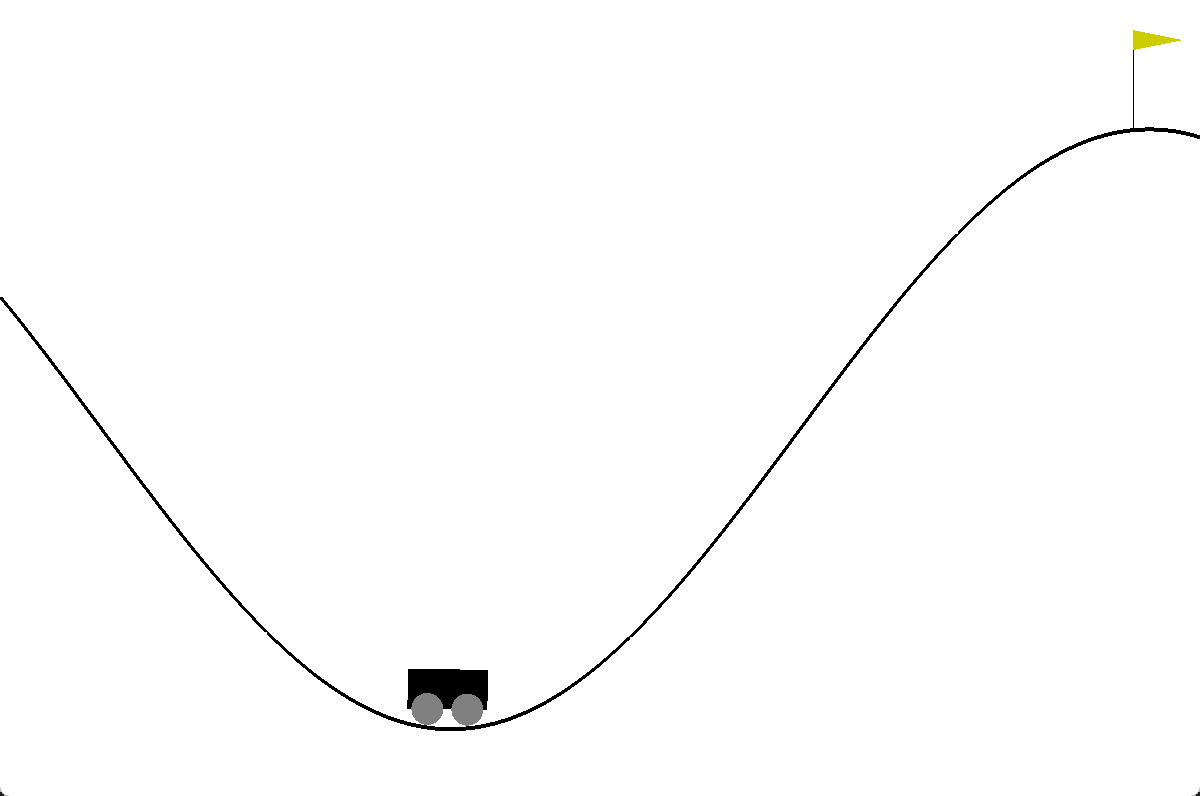
\includegraphics[width=0.5\linewidth]{MountainCar.png}
    \caption{What the Mountain Car environment looks like. The car starts at some point in the valley. The goal is to get to the top right flag.}
    \label{fig:mountaincar}
\end{figure}

The state of the environment is represented by two variables, \texttt{position} and \texttt{velocity}. \texttt{position} can be between $[-1.2, 0.6]$ (inclusive) and \texttt{velocity} can be between $[-0.07, 0.07]$ (inclusive). These are just measurements along the $x$-axis.

The actions that you may take at any state are $\{0, 1, 2\}$, where each number corresponds to an action: (0) pushing the car left, (1) doing nothing, and (2) pushing the car right.

\subsection{Q-learning with Linear Approximations}
The Q-learning algorithm is a model-free reinforcement learning algorithm, where we assume we don't have access to the model of the environment the agent is interacting with. We also don't build a complete model of the environment during the learning process. A learning agent interacts with the environment solely based on calls to \textbf{step} and \textbf{reset} methods of the environment. Then the Q-learning algorithm updates the q-values based on the values returned by these methods. Analogously, in the approximation setting the algorithm will instead update the parameters of q-value approximator.


Let the learning rate be $\alpha$ and discount factor be $\gamma$. Recall that we have the information after one interaction with the environment, $(s, a, r, s')$. The tabular update rule based on this information is: 
\[
    Q(s,a) = (1 - \alpha) Q(s, a) + \alpha \left(r + \gamma \max_{a'} Q(s', a')\right).
\]

Instead, for the function approximation setting we use the following update rule derived from the Function Approximation Section (Section \ref{sec:FA}). Note that we have made the bias term explicit here, where before it was implicitly folded into $\wv$:
\[
\wv \leftarrow \wv - \alpha \left(q(\sv, a; \wv) - (r + \gamma \max_{a'} q(\sv', a'; \wv)\right) \nabla_\wv q(\sv, a; \wv),
\]
where
\[
q(\sv,a;\wv) = \sv^T \wv_a + b.
\]
The epsilon-greedy action selection method selects the optimal action with probability $1 - \epsilon$ and selects uniformly at random from one of the 3 actions ($0$, $1$, $2$) with probability $\epsilon$. The reason that we use an epsilon-greedy action selection is we would like the agent to do explorations by stochastically selecting random actions with small probability. For the purpose of testing, we will test two cases: $\epsilon = 0$ and $0 < \epsilon < 1$. When $\epsilon = 0$ (no exploration), the program becomes deterministic and your output have to match our reference output accurately. In this case, \textbf{pick the action represented by the smallest number if there is a draw in the greedy action selection process}. For example, if we are at state $s$ and $Q(s, 0) = Q(s, 2)$, then take action $0$. When $0 < \epsilon < 1$, your output will need to fall in a certain range within the reference determined by running exhaustive experiments on the input parameters.


\subsection{Feature Engineering}
Linear approximations are great in their ease of use and implementations. However, there sometimes is a downside; they're \emph{linear}. This can pose a problem when we think the value function itself is nonlinear with respect to the state. For example, we may want the value function to be symmetric about 0 velocity. To combat this issue we could throw a more complex approximator at this problem, like a neural network. But we want to maintain simplicity in this assignment, so instead we will look at a nonlinear transformation of the ``raw'' state.

\begin{figure}[H]
\centering
\begin{subfigure}{0.5\textwidth}

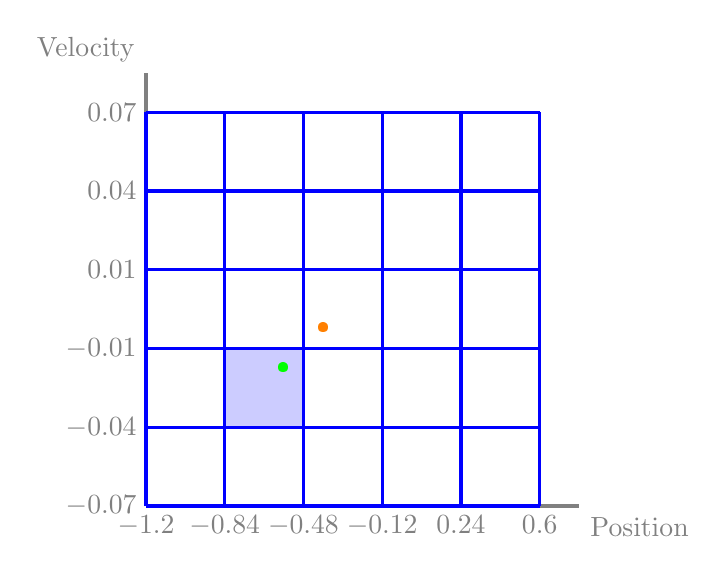
\begin{tikzpicture}[scale=1.0]
% https://tex.stackexchange.com/questions/45808/tikz-grid-lines
% https://tex.stackexchange.com/questions/305138/modify-the-scale-of-x-axis-and-y-axis
\pgfkeys{/pgf/number format/.cd,fixed,precision=2}
% Draw labels
\draw [ultra thick,gray,] (0,0)--(5.5,0) node[below right] {\text{Position}};
\draw [ultra thick,gray,] (0,0)--(0,5.5) node[above left] {\text{Velocity}};
% Draw axis
\newcommand*{\xMin}{0}%
\newcommand*{\xMax}{5}%
\newcommand*{\yMin}{0}%
\newcommand*{\yMax}{5}%
    \foreach \i in {\xMin,...,\xMax} {
        \draw [very thin,gray] (\i,\yMin) -- (\i,\yMax)  node [below] at (\i,\yMin) {\pgfmathparse{(\i/50)*18-1.2}$\pgfmathprintnumber{\pgfmathresult}$};
    }
    \foreach \i in {\yMin,...,\yMax} {
        \draw [very thin,gray] (\xMin,\i) -- (\xMax,\i) node [left] at (\xMin,\i) {\pgfmathparse{(\i/500)*14-0.07}$\pgfmathprintnumber{\pgfmathresult}$};
    }
% Draw grids
\draw [step=1.0,blue, very thick] (0.0,0.0) grid (5.0,5.0);
% \draw [very thick, red, step=1.0cm,xshift=-0.5cm, yshift=-0.5cm] (0.5,0.5) grid +(5.0,5.0);

% Draw shaded regions
\fill [blue, opacity=0.2] (1,1) rectangle (2,2);
% \fill [red, opacity=0.2] (1.5,1.5) rectangle (2.5,2.5);

% Draw point
\node [green] at (1.75,1.75) {\textbullet};
\node [orange] at (2.25, 2.25) {\textbullet};

\end{tikzpicture}
\caption{A discretization of the state space of Mountain Car}
\label{fig:discrete}
\end{subfigure}%
\begin{subfigure}{0.5\textwidth}

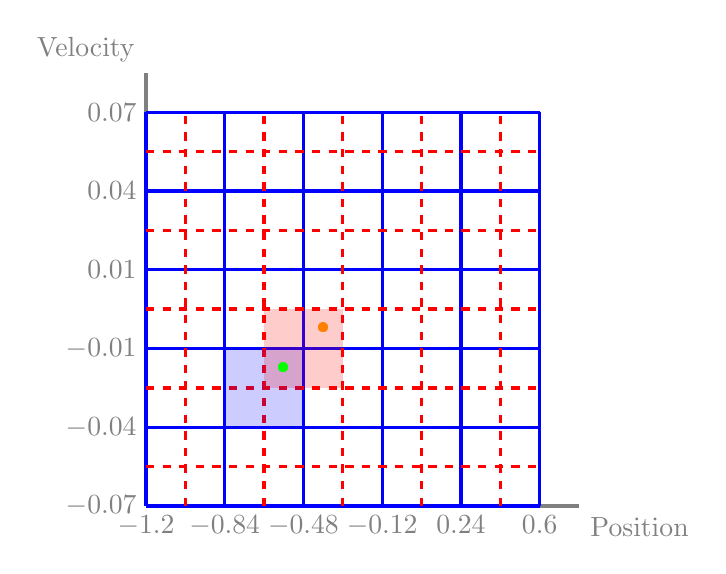
\begin{tikzpicture}[scale=1.0]
% https://tex.stackexchange.com/questions/45808/tikz-grid-lines
% https://tex.stackexchange.com/questions/305138/modify-the-scale-of-x-axis-and-y-axis
\pgfkeys{/pgf/number format/.cd,fixed,precision=2}
% Draw labels
\draw [ultra thick,gray,] (0,0)--(5.5,0) node[below right] {\text{Position}};
\draw [ultra thick,gray,] (0,0)--(0,5.5) node[above left] {\text{Velocity}};
% Draw axis
\newcommand*{\xMin}{0}%
\newcommand*{\xMax}{5}%
\newcommand*{\yMin}{0}%
\newcommand*{\yMax}{5}%
    \foreach \i in {\xMin,...,\xMax} {
        \draw [very thin,gray] (\i,\yMin) -- (\i,\yMax)  node [below] at (\i,\yMin) {\pgfmathparse{(\i/50)*18-1.2}$\pgfmathprintnumber{\pgfmathresult}$};
    }
    \foreach \i in {\yMin,...,\yMax} {
        \draw [very thin,gray] (\xMin,\i) -- (\xMax,\i) node [left] at (\xMin,\i) {\pgfmathparse{(\i/500)*14-0.07}$\pgfmathprintnumber{\pgfmathresult}$};
    }
% Draw grids
\draw [step=1.0,blue, very thick] (0.0,0.0) grid (5.0,5.0);
\draw [very thick, dashed, red, step=1.0cm,xshift=-0.5cm, yshift=-0.5cm] (0.5,0.5) grid +(5.0,5.0);

% Draw shaded regions
\fill [blue, opacity=0.2] (1,1) rectangle (2,2);
\fill [red, opacity=0.2] (1.5,1.5) rectangle (2.5,2.5);

% Draw point
\node [green] at (1.75,1.75) {\textbullet};
\node [orange] at (2.25, 2.25) {\textbullet};

\end{tikzpicture}
\caption{A tiling of the state space of Mountain Car}
\label{fig:tiling}
\end{subfigure}

\caption{State representations for the states of Mountain Car}
\label{fig:states}
\end{figure}

For the Mountain Car environment, we know that \texttt{position} and \texttt{velocity} are both bounded. What we can do is draw a grid over the possible \texttt{position}-\texttt{velocity} combinations as seen in Figure~\ref{fig:discrete}. We then enumerate the grid from bottom left to top right, row by row. Then we map all states that fall into a grid square with the corresponding one-hot encoding of the grid number. For efficiency reasons we will just use the index that is non-zero. For example the green point would be mapped to $\{6\}$ and the orange point to $\{12\}$. This is called a \emph{discretization} of the state space.

The downside to the above approach is that although observing the green point will let us learn parameters that generalize to other points in the shaded blue region, we will not be able to generalize to the orange point even though it is nearby. We can instead draw two grids over the state space, each offset slightly from each other as in Figure~\ref{fig:tiling}. Now we can map the green point to two indices, one for each grid, and get $\{6, 39\}$ (note the index for orange grid starts from the end of blue index, i.e. $25$). Now the green point has parameters that generalize to points that map to $\{6\}$ (the blue shaded region) in the first discretization and parameters that generalize to points that map to $\{39\}$ (the red shaded region) in the second. We can generalize this to multiple grids, which is what we do in practice. This is called a \emph{tiling} or a \emph{coarse-coding} of the state space. 


\subsection{Implementation Details}
Here we describe the API to interact with the Mountain Car environment available to you.

\begin{itemize}
    \item \texttt{\_\_init\_\_(mode, debug)}: Initializes the environment to the a mode specified by the value of \texttt{mode}. This can be a string of either ``raw'' or ``tile''. 
    
    ``raw'' mode tells the environment to give you the state representation of raw features encoded in a sparse format: $\{0 \rightarrow \texttt{position}, 1 \rightarrow \texttt{velocity}\}$.
    
    In ``tile'' mode you are given indices of the tiles which are active in a sparse format: $\{T_1 \rightarrow 1, T_2 \rightarrow 1, \ldots T_n \rightarrow 1\}$ where $T_i$ is the tile index for the $i$th tiling. All other tile indices are assumed to map to 0. For example the state representation of the example in Figure~\ref{fig:tiling} would become $\{6 \rightarrow 1, 39 \rightarrow 1\}$.
    
    The dimension of the state space of the ``raw'' mode is 2. The dimension of the state space of the ``tile'' mode is 2048. These values can be accessed from the environment through the \texttt{state\_space} property, and similarly for other languages.
    
    \texttt{debug} is an optional argument for debugging. See Section \ref{subsec:debugging} for more details.
    
    \item \texttt{reset()}: Reset the environment to starting conditions.
        \item \texttt{step(action)}: Take a step in the environment with the given action. \texttt{action} must be either $0$, $1$ or $2$. This will return a tuple of $(\texttt{state}, \texttt{reward}, \texttt{done})$ which is the next state, the reward observed, and a boolean indicating if you reached the goal or not, ending the episode. The \texttt{state} will be either a raw' or tile representation, as defined above, depending on how you initialized Mountain Car.  If you observe \texttt{done = True} then you should \texttt{reset} the environment and end the episode. Failure to do so will result in undefined behavior.
    \item \texttt{render()}: Visualize the environment (not graded). Requires the installation of \texttt{pyglet}\footnote{You can install it by typing \texttt{pip install pyglet} in your shell.}. We highly recommend you to use this only after you implement everything. Do \emph{not} use this as a tool for debugging---this should rather be used as a tool for understanding Q-learning better. It is computationally intensive to render graphics, so only call the function once every 100 or 1000 episodes. This will be a no-op in Gradescope.
\end{itemize}

You should now implement your Q-learning algorithm with linear approximations in \texttt{q\_learning.py}. The program will assume access to a given environment file(s) which contains the Mountain Car environment which we have given you.  \textbf{Initialize the parameters of the linear model with all 0 (and don't forget to include a bias!) and use the epsilon-greedy strategy for action selection.}

Your program should write a output file containing the total rewards (the returns) for every episode after running Q-learning algorithm. There should be one return per line.

Your program should also write an output file containing the weights of the linear model. The first line should be the value of the bias. Then the following $|\mathcal{S}| \times |\mathcal{A}|$ lines should be the values of weights, outputted in row major order\footnote{\url{https://en.wikipedia.org/wiki/Row-_and_column-major_order}}, assuming your weights are stored in a $|\mathcal{S}| \times |\mathcal{A}|$ matrix.

The autograder will use the following commands to call your function:

\begin{tabbing}
\=\texttt{\$ \textbf{python} q\_learning.\textbf{py} [args\dots]}
\end{tabbing}

where above \texttt{[args\dots]} is a placeholder for command-line arguments: \texttt{<env>} \texttt{<mode>} \texttt{<weight\_out>} \texttt{<returns\_out>} \texttt{<episodes>} \texttt{<max\_iterations>} \texttt{<epsilon>} \texttt{<gamma>} \texttt{<learning\_rate>}. These arguments are described in detail below:
\begin{enumerate}
    \item \texttt{<env>}: the environment that you are running, either \texttt{mc} for Mountain Car or \texttt{gw} for Grid World.
    \item \texttt{<mode>}: mode to run the environment in. Should be either \texttt{raw} or \texttt{tile}. Note that Grid World operates only in \texttt{tile} mode.
    \item \texttt{<weight\_out>}: path to output the weights of the linear model.
    \item \texttt{<returns\_out>}: path to output the returns of the agent.
    \item \texttt{<episodes>}: the number of episodes your program should train the agent for. One episode is a sequence of states, actions and rewards, which ends with terminal state or ends when the maximum episode length has been reached.
    \item \texttt{<max\_iterations>}: the maximum of the length of an episode. When this is reached, we terminate the current episode.
    \item \texttt{<epsilon>}: the value $\epsilon$ for the epsilon-greedy strategy.
    \item \texttt{<gamma>}: the discount factor $\gamma$.
    \item \texttt{<learning\_rate>}: the learning rate $\alpha$ of the Q-learning algorithm.
\end{enumerate}


Example command:
\begin{lstlisting}[language=Shell]
$ python q_learning.py mc raw mc_raw_weight.out mc_raw_returns.out \ 
 4 200 0.05 0.99 0.01
\end{lstlisting}

Example output from the above command (may not be exactly the same, but should be close up to 0.01):

\texttt{<weight\_out>}
\begin{lstlisting}
-7.66116708660012
1.3411763263964611
1.3419332653944924
1.3370748857368524
-0.0013201697867872468
0.0010668243394517697
0.0012565450062079566
\end{lstlisting}

\texttt{<returns\_out>}
\begin{lstlisting}
-200.0
-200.0
-200.0
-200.0
\end{lstlisting}


\subsection{Debugging Tips}\label{subsec:debugging}

To help with debugging, we have provided the option for printing each step of the Q-learning train function based on the reference output for the Grid World environment. We created this output by adding the \texttt{debug=True} argument when initializing the Grid World environment. You may do the same to compare your output against ours.

We recommend first checking your outputs based on a run with extremely simple parameters. Remember to set \texttt{<epsilon>=0} so the program is run without the epsilon-greedy strategy.

We have provided output on the Grid World for the following simple command:

\begin{lstlisting}[language=Shell]
$ python q_learning.py gw tile gw_simple_weight.out \
  gw_simple_returns.out 1 1 0.0 1 1
\end{lstlisting}

Once this works, you can change the parameters to be slightly more complex (such as the ones we have below), and check with our calculations again:

\begin{lstlisting}[language=Shell]
$ python q_learning.py gw tile gw_weight.out gw_returns.out \
  3 5 0.0 0.9 0.01
\end{lstlisting}

The logs for both of the above commands should be in \texttt{reference\_output/gw\_simple.log} and \texttt{reference\_output/gw.log}, respectively.

In addition, we have provided \texttt{mc\_weight.out} and \texttt{mc\_returns.out} in the handout, which are generated using the following parameters:
\begin{itemize}
    \item \texttt{<env>}: \texttt{mc}
    \item \texttt{<mode>}: \texttt{tile}
    \item \texttt{<episodes>}: \texttt{25}
    \item \texttt{<max\_iterations>}: \texttt{200}
    \item \texttt{<epsilon>}: \texttt{0.0}
    \item \texttt{<gamma>}: \texttt{0.99}
    \item \texttt{<learning\_rate>}: \texttt{0.005}
\end{itemize}

Example command:
\begin{lstlisting}[language=Shell]
$ python q_learning.py mc tile mc_tile_weight.out \
 mc_tile_returns.out 25 200 0.0 0.99 0.005
\end{lstlisting}

\subsection{Gradescope Submission}

You should submit your \texttt{q\_learning.py} to Gradescope.
\textbf{Any other files uploaded will be discarded or reverted back to the original version provided in the handout.}
Do \textit{not} use other file names.
\end{document}
